\documentclass[czech,bachelor]{../../shared/diploma}

\usepackage[autostyle=true,czech=quotes]{csquotes} % korektni sazba uvozovek, podpora pro balik biblatex
\usepackage[backend=biber, style=iso-numeric, alldates=iso]{biblatex} % bibliografie
\usepackage{dcolumn} % sloupce tabulky s ciselnymi hodnotami
\usepackage{subfig} % makra pro "podobrazky" a "podtabulky"
\usepackage{float} % lepsi umistovani obrazku (H)
\usepackage{subcaption}
\usepackage{hyperref}
\usepackage{listings}
\usepackage{tikz}
\usepackage{color} % Required for custom colors
\usepackage{bookmark} % Required for generating PDF bookmarks

\definecolor{darkgreen}{rgb}{0,0.6,0}
\definecolor{gray}{rgb}{0.5,0.5,0.5}
\definecolor{mauve}{rgb}{0.58,0,0.82}

\renewcommand{\lstlistingname}{Zdrojový Kód} % Set your own caption name for listings

\newenvironment{plantuml}[1]{\VerbatimOut{#1.puml}}{\endVerbatimOut}
\newcommand{\processDiagram}[4]{%
    \IfFileExists{../../mik0486/target/puml/#2.pdf}{%
        \ifnum\pdfstrcmp{\pdffilemoddate{../../mik0486/target/puml/#2.pdf}}{\pdffilemoddate{#1.puml}}<0
            \immediate\write18{java -jar ../../shared/libs/plantuml-1.2024.3.jar -o ../../../mik0486/target/puml -tsvg #1.puml}
            \immediate\write18{inkscape ../../mik0486/target/puml/#2.svg --export-area-drawing --export-filename=../../mik0486/target/puml/#2.pdf}
        \fi
    } {%
        \immediate\write18{java -jar ../../shared/libs/plantuml-1.2024.3.jar -o ../../../mik0486/target/puml -tsvg #1.puml}
        \immediate\write18{inkscape ../../mik0486/target/puml/#2.svg --export-area-drawing --export-filename=../../mik0486/target/puml/#2.pdf}
    }

    \begin{figure}[H]
        \centering
        \includegraphics[width=#3]{../../mik0486/target/puml/#2}
        \caption{#4}\label{fig:figure}
    \end{figure}
}

\lstdefinelanguage{CSS}{
    sensitive=true,
    keywords={color:, background-color:, margin:, padding:, font:, weight:, display:, position:, top:, left:, right:, bottom:, list:, style:, border:},
    morecomment=[l]{//},
    morecomment=[s]{/*}{*/},
    morestring=[b]',
    morestring=[b]",
    alsoletter={:},
    alsodigit={-}
}

\lstdefinelanguage{HTML}{
    sensitive=true,
    keywords={html,head,title,meta,script,style,link,body,h1,h2,h3,h4,h5,h6,p,div,span,a,img,ul,ol,li,table,th,tr,td,thead,tbody,tfoot,form,input,button,select,option,label,textarea},
    morecomment=[s]{<!--}{-->}
}

\lstset{
    basicstyle=\ttfamily\small,     % The basic style
    keywordstyle=\color{blue},      % Keyword style
    commentstyle=\color{darkgreen}, % Comment style
    stringstyle=\color{mauve},      % String literal style
    breaklines=true,                % Break long lines
    showstringspaces=false,         % Don't show spaces in strings as special character
    numbers=left,                   % Line numbers on the left
    numberstyle=\tiny\color{gray},  % Style of line numbers
    tabsize=2,                      % Set tab size
    frame=l,                        % Left frame line
    framesep=5pt,                   % Padding between frame and code
    xleftmargin=\parindent,         % Indent the frame to fit paragraph layout
    captionpos=b,                   % Position the caption at the bottom
    aboveskip=1em,                  % Adjust the space above the listing
    literate={á}{{\'{a}}}1 {Á}{{\'{A}}}1 {ä}{{\"{a}}}1 {Ä}{{\"{A}}}
    1 {č}{{\v{c}}}1 {Č}{{\v{C}}}1 {ď}{{\v{d}}}1 {Ď}{{\v{D}}}
    1 {ě}{{\v{e}}}1 {Ě}{{\v{E}}}1 {é}{{\'{e}}}1 {É}{{\'{E}}}
    1 {í}{{\'{i}}}1 {Í}{{\'{I}}}1 {ĺ}{{\'{l}}}1 {Ĺ}{{\'{L}}}
    1 {ľ}{{\v{l}}}1 {Ľ}{{\v{L}}}1 {ň}{{\v{n}}}1 {Ň}{{\v{N}}}
    1 {ó}{{\'{o}}}1 {Ó}{{\'{O}}}1 {ô}{{\^{o}}}1 {Ô}{{\^{O}}}
    1 {ř}{{\v{r}}}1 {Ř}{{\v{R}}}1 {ŕ}{{\'{r}}}1 {Ŕ}{{\'{R}}}
    1 {š}{{\v{s}}}1 {Š}{{\v{S}}}1 {ť}{{\v{t}}}1 {Ť}{{\v{T}}}
    1 {ú}{{\'{u}}}1 {Ú}{{\'{U}}}1 {ů}{{\r{u}}}1 {Ů}{{\r{U}}}
    1 {ý}{{\'{y}}}1 {Ý}{{\'{Y}}}1 {ž}{{\v{z}}}1 {Ž}{{\v{Z}}}1
}

% Pozadovane vstupy pro generovani titulnich stran.
\ThesisAuthor{Pavel Mikula}
\ThesisSupervisor{Ing. Radoslav Fasuga, Ph.D.}
\CzechThesisTitle{Tvorba administrativního rozhraní výpravné evoluční hry}
\EnglishThesisTitle{Creation of the Administrative Interface for the Narrative Evolution Game}
\SubmissionYear{2024}

\ThesisAssignmentFileName{../specification.pdf}

\CzechAbstract{
    Tato bakalářská práce se zabývá tvorbou administrativního rozhraní pro správu obsahu výpravné evoluční hry, kde rozhraní umožňuje
    kompletní operace nad objekty jako jsou postavy, předměty, lokace, události a další. Pro vytvoření administrativního rozhraní je nutné
    provést analýzu možných rozhraní, návrh a následnou implementaci. Jako finální produkt práce by měl vzniknout funkční prototyp
    administrativní rozhraní, který bude umožňovat kompletní správu obsahu pomocí napojení na webové API, které bude poskytovat
    data přímým přístupem k databázi.
}
\CzechKeywords{administrativní rozhraní, výpravně evoluční hra, správa obsahu hry, vykreslování, interaktivní editor}

% TODO: Zkontrolovat, zda je abstrakt v angličtině správný, by AI
\EnglishAbstract{
    This bachelor thesis focuses on the development of an administrative interface for managing the content of an narrative evolutionary game.
    The interface enables comprehensive content management, including characters, items, locations, events, and more.
    To create the administrative interface, it is necessary to perform an analysis of possible interfaces, design a solution,
    and subsequently implement it. The final product of this work should be a functional prototype of the administrative interface,
    allowing complete content management through integration with a web API providing direct access to the database.
}
\EnglishKeywords{administrative interface, expansive evolutionary game, game content management, rendering, interactive editor}

% TODO: Zkontrolovat všechny zkratky v dokumentu
\AddAcronym{API}{Aplikační programové rozhraní}
\AddAcronym{JS}{JavaScript}
\AddAcronym{HTML}{Hyper Text Markup Language}

\Acknowledgement{
    Rád bych na tomto místě poděkoval vedoucímu práce Ing. Radoslavu Fasugovi, Ph.D. za jeho cenné rady, trpělivost a ochotu věnovat mi svůj čas.
    Dále bych chtěl poděkovat svým kolegům Martinu Korotwitschkovi, Barboře Kovalské a Miroslavu Osobovi za jejich asistenci při vývoji.
}

% Novy druh tabulkoveho sloupce, ve kterem jsou cisla zarovnana podle desetinne carky
\newcolumntype{d}[1]{D{,}{,}{\#1}}

\addbibresource{resources/sauce.bib}

% Uprava hloubky obsahu - pozdeji smazat !
\setcounter{tocdepth}{3}

% Zacatek dokumentu
\begin{document}

% Titulni strany
\MakeTitlePages

% Obrazky
\listoffigures
\clearpage

% Tabulky
\listoftables
\clearpage

% Úvod
\chapter{Úvod}

Welcome to hell. This is the introduction chapter.

% Kapitoly
\chapter{Teorie a analýza}
\label{ch:theory_and_analysis}
V této kapitole se budeme věnovat teorii a analýze rozhraní, včetně jejich klíčových prvků, které jsou zásadní pro pochopení základních principů efektivního designu jak uživatelských (UI), tak i administrativních rozhraní. Dále se zaměříme na analýzu populárních deskových her, které si v současné době získaly velkou popularitu a zájem hráčů. V závěru této kapitoly se zaměříme na administrativní prvky a značky, které jsou zásadní pro správu obsahu aplikace.

\section{Teorie UI/GUI}
\label{sec:ui-gui-theory}
Uživatelské rozhraní z anglického jazyka \textit{\textquote{User Interface}} (UI) a grafické uživatelské rozhraní \textit{\textquote{Graphical User Interface}} (GUI) jsou termíny používány v kontextu digitálních aplikací, kde tyto komponenty umožňují uživatelům interagovat se softwárem aplikace pomocí rozhraní. Zatímco UI zahrnuje jakoukoliv formu uživatelského rozhraní, GUI se specificky zaměřuje na vizuální aspekty rozhraní jako jsou okna, ikony, tlačítka a další grafické elementy.

Základem dobrého UI je především jeho intuitivita, jednoduchost a přehlednost, což jednoduše znamená, že by uživatel měl být schopen jednoduše pochopit jak s aplikačním rozhraním pracovat, aniž by musel procházet složitějším procesem učení.

\subsection*{Klíčové prvky UI/GUI}
\label{subsec:ui-gui-theory-key-elements}
\begin{itemize}
    \item \textbf{Rozložení} -- Efektivní rozložení usnadňuje uživatelskou orientací, uživatelé pak snadnější naleznou potřebné funkce nebo informace.
    \item \textbf{Prvky ovládání} -- Tlačítka, menu, přepínače a další administrativní prvky by měly být v ideálním případě jasně označené a snadno dostupné.
    \item \textbf{Typografie a barevnost} -- Výběr písma a jeho barevné schéma hraje významnou roli v čitelnosti a celkovém vnímání. V dnešní době se stránky hodně zaměřují na tmavá přepínatelná pozadí často známá jako \textit{Dark Mode} a \textit{Light Mode}.
    \item \textbf{Interaktivita} -- Při podání vstupu do aplikace by uživatelé měli dostat okamžitou zpětnou vazbu, čímž tak dostávají informace, že jejich akce byla zpracována nebo se aktuálně zpracovává. Často je tak probíhající akce vyobrazena určitým opakujícími se animacemi například tak točící se kolečko známé jako \textit{loading spinner}.
    \item \textbf{Přizpůsobivost} -- Možnost přizpůsobit si uživatelské rozhraní tak zvyšuje celkovou přívětivost, v rozhraních tak většinou nalezneme možnost změnit jazyk, barvy nebo pozice jednotlivých oken. Tyto změny se tak většinou uchovávají pouze v uložišti prohlížeče a nejsou nijak sdílený mezi zařízeními.
\end{itemize}

\subsection*{Principy dobrého UI designu}
\label{subsec:ui-gui-theore-basic-use-case}
\begin{itemize}
    \item \textbf{Konzistence} -- Při provádění stejné akce, by uživatel měl pokaždé dostat stejnou odpověď.
    \item \textbf{Jednoduchost} -- UI by mělo mít minimalistický design, který je hlavně zaměřen na důležité funkce.
    \item \textbf{Přívětivost} -- Uživatel by měl být schopen, okamžitě pochopit rozložení UI bez nutnosti se ho učit.
    \item \textbf{Dostupnost} -- UI by mělo být dostupné pro všechny uživatele, bez ohledu na jejich schopnosti.
    \item \textbf{Zabezpečení} -- UI by mělo být zabezpečené a chránit uživatele před různými útoky.
\end{itemize}

\subsection{Počátek vzniku rozhraní}
\label{subsec:ui-gui-theory-beginning}
Vznik rozhraní lze vysledovat až k raným počátkům počítačů, kde se interakce mezi uživatelem a rozhraním prováděla pomocí děrných štítků a přepínačů. Postupem času s vývojem technologií vzniklo rozhraní terminálové z anglického jazyka \textit{\textquote{Command Line Interface}} (CLI), které obsahovalo základní textový vstup z klávesnice a následného výstupu umístěného na displej. Toto rozhraní se tak stalo standardem pro každý novodobý počítač a používá se do dnešních let. Zlomovým momentem se poté stal příchod grafické rozhraní z angl. \textit{\textquote{Graphical User Interface}} (GUI), které znamenalo revoluci v přístupu k interakci uživatele s počítačem. Tato evoluce přinesla nové možnosti pro uživatele jak přímo komunikovat s počítačem díky grafickým prvkům jako jsou okna, ikony, menu za pomocí pohybu myši po obrazovce.

Pro nás se grafická reprezentace v počítači stala již nedílnou součástí našeho života a v dnešní době se sní setkáváme již na každém kroku, ať se jedná o mobilní aplikace, počítačové aplikace nebo prosté webové stránky.

Pro vývoj webových aplikací se většinou používají technologie spojené pomocí jazyku JavaScript. V minulých letech, zde ale existoval software se jménem \textit{Adobe Flash Player}, který umožňoval vytvářet interaktivní multimediální obsah, které se mnohdy využíval na vývoj různých webových aplikace ať se jednalo o různé hry, prezentace nebo třeba aplikaci fotogalerie. Bohužel tento software byl koncem roku 2020 ukončen a nahrazen modernějšími a bezpečnějšími technologiemi, které zároveň stály za jeho úpadkem. Mezi tyto technologie se tak řadí HTML5, WebGL nebo WebAssembly. \cite{adobeFlashPlayer-eol}

\subsection{Problematika vývoje}
\label{subsec:ui-gui-theory-problems}
Problematika vývoje rozhraní se týká komplexního procesu, který zahrnuje několik oblastí, nad kterými je potřeba se předem zamyslet a následně je implementovat. Většinou při zanedbaní správné implementace těchto sekcí, lze v budoucnu rychle dosáhnout problémům, kde jejich řešení může mít výrazný vliv na funkčnost aplikace. Mezi tyto oblasti spadá například:

\begin{itemize}
    \item \textbf{Uživatelský vstup}, který reprezentuje jakým způsobem bude uživatel nebo administrátor aplikaci podávat vstup. Tedy jestli se jedná o textový vstup, vstup ovládáním myši nebo dotykovým displejem. Dle tohoto kritéria se poté volí vhodný způsob zpracování vstupu.
    \item \textbf{Vykreslování}, které se většinou rozděluje na potřeby uživatelské a administrativní částí. Kde uživatelská se zaměřuje více na design a přívětivost pro uživatele, zatímco administrativní se zaměřuje na efektivitu a snadnou správu obsahu. Tento rozdíl můžeme jednoduše vidět na tom, že administrativní rozhraní často využívá plný potenciál obrazovky, zatímco uživatelské se snaží dbát na přehlednost a jednoduchost.
    \item \textbf{Responzivní design} určuje, jak se jednotlivé prvky v obrazovce zachovají při změně velikosti okna nebo zařízení. Aplikace by v ideálním případě po změně velikosti neměla ztratit na přehlednosti nebo jakkoliv poškodit uživatelskou zkušenost. U mobilních verzí aplikací se tak často objevují separátní odkazy na nativní rozhraní, které se tak často nachází pod subdoménou s název \("\)m\("\) tedy například \textit{https://m.tts-game.fun}. Řešení responzivního designu dále bude pokračovat v separátním odstavci~\ref{subsec:ui-gui-theory-responsive-design}.
    \item \textbf{Uživatelská zkušenost} z anglického jazyka \textit{\textquote{User Experience}} (UX) se soustředí na to, jak uživatelé vnímají a jak se cítí při používání aplikace. Tedy jak je aplikace přívětivá, snadno ovladatelná a zda splňuje očekávání uživatele.
    \item \textbf{Bezpečnost} je důležitým aspektem, který se zaobírá zpracováním uživatelských dat, které v mnoha případech obsahuje citlivé informace. Při nesprávném zpracování těchto dat může dojít k úniku dat nebo zneužití. Jako řešení se používají různé techniky, jako je například šifrování, ověřování uživatele nebo zabezpečení připojení.
\end{itemize}

\subsection{Responzivní design}
\label{subsec:ui-gui-theory-responsive-design}
Responzivní design se stal již skoro povinným standardem pro všechny webové stránky a aplikace. Tento přístup se zaměřuje na webové prvky tak, aby při jejich zobrazení na různých zařízeních s rozdílnou velikosti obrazovky nebo orientace byly pořád stejně přehledné a plně funkční. Této funkčnosti se dosahuje pomocí CSS stylů, které tuto funkcionalitu umožňují pomocí tzv. \textit{\textquote{media queries}}. Tyto dotazy umožňují nastavovat styly podle předem daných kritérii, jako jsou například šířka okna, výška okna, typ zařízení nebo jeho orientace.

Jedním z průkopníků responzivního designu se stal \textit{Bootstrap}, open-source framework pro vývoj front-end webových aplikací. Který nabízí soubor knihoven a předem vytvořených šablon stylů, díky kterým je možné za použití pár elementů dosáhnout rychlého a plně responzivního designu aplikace. Tento framework je v současné době jedním z nejpoužívanějších z důvodu jeho lehkého nasazení, široké podpory a velké kompatibility. Využití potenciálu tohoto frameworku si blíže popíšeme v kapitole~\ref{subsec:dev-technology-bootstrap}.

\lstinputlisting[language=CSS, caption={Příklad použití media query v css.}, label={lst:media-query-example}]{sourceCodes/MediaQueryExample.css}

V stručném vysvětlení kódu~\ref{lst:media-query-example} můžeme vidět, že se jedná o základní CSS kód, který nastavuje barvu pozadí stránky na světle šedou. Ale obsahuje media dotaz na řádku 6, které se ptá na velikost obrazovky, kde v případě, že je šířka obrazovka menší než 600px, změní barvu pozadí na světle modrou.

\begin{figure}[H]
    \centering
    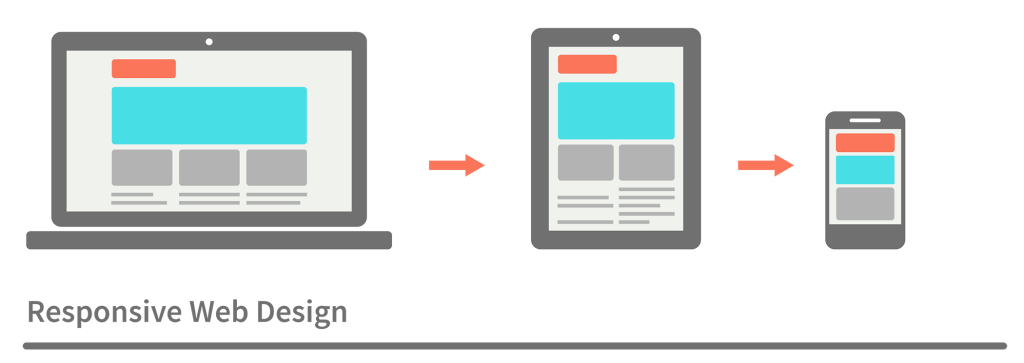
\includegraphics[width=1.0\textwidth]{figures/responsiveDesign}
    \caption{Ukázka responzivního designu mezi zařízeními. \cite{responsive_design}}
    \label{fig:responsive-design-example}
\end{figure}

\section{Analýza populárních deskových her}
\label{sec:popular-board-games-analysis}
Deskových her je v dnešní době na trhu velké množství, kde každým rokem se snaží noví nebo i stálí autoři proniknout ven s novými nápady nebo koncepty. Deskové hry lze tak rozdělit na několik herních žánru, jako jsou například hry strategické, kooperativní, party, rodinné nebo třeba karetní. Velká většina z těchto her se zaměřuje na její plný průběh na půdě hracího stolu, existují zde ale i hry, které do tohoto průběhu zapojují i externí zařízení, jako jsou speciální zařízení, mobilní telefony nebo laptopy. Tyhle hry se nazývají hry hybridní, kde jejich bližší definici popíšu v následující sekci.

\subsection*{Hybridní hry}
\label{subsec:popular-board-games-analysis-hybrid-games}
Jak již bylo zmíněno o sekci výše, hybridní hry jsou hry takové, které kombinují jednotlivé funkční prvky z her fyzických nebo digitálních. Jednoduše se tak dá řici, že hybridní hra je hra taková, které má jakékoliv napojení na technologii. Mezi hry hybridní tak patří například populární hra \textit{Monopoly}, která použivá speciální bankovní zařízení používané pro správu financí nebo hra \textit{XCOM: The Board Game}, která využívá mobilní aplikaci pro správu herního průběhu.

\subsection{Populární deskové hry}
\label{subsec:popular-board-games-analysis-popular-games}
Populárních deskových her je na světě velké množství, pro tuto analýzu jsem si vybral několik her, které mi jsou nejbližší a již jsem měl možnost si je zahrát. Díky této zkušenosti můžu lépe popsat možnosti a prvky, které tyto hry obsahují. Mezi tyto stolní hry patří například \textit{Carcassonne}, \textit{Bang!}, \textit{Codenames} nebo \textit{Gloomhaven}.

\subsubsection{Carcassonne}
\label{subsubsec:popular-board-games-analysis-carcassonne}
\textcolor{red}{DOPLNIT -- Popsat hru jak funguje, cíl, jaké prvky obsahuje, rozšíření. Poté její online verze.}

\subsubsection{Bang!}
\label{subsubsec:popular-board-games-analysis-bang}
\textcolor{red}{DOPLNIT -- Popsat hru jak funguje, cíl, jaké prvky obsahuje, rozšíření. Poté její online verze.}

\subsubsection{Codenames (Krycí jména)}
\label{subsubsec:popular-board-games-analysis-codenames}
\textcolor{red}{DOPLNIT -- Popsat hru jak funguje, cíl, jaké prvky obsahuje, rozšíření. Poté její online verze.}

\subsubsection{Gloomhaven}
\label{subsubsec:popular-board-games-analysis-gloomhaven}
\textcolor{red}{DOPLNIT -- Popsat hru jak funguje, cíl, jaké prvky obsahuje, rozšíření. Poté její online verze.}

\section{Administrativní prvky}
\label{sec:admin-elements}
Každé administrativní rozhraní se skládá z několika základních prvků, které umožňuje uživatelům s administrativními oprávněním provádět specifické úkony nebo měnit kompletní nastavení aplikace. Mezi takové prvky patří například správa uživatelů, obsahu, nastavení, zobrazení statistik nebo přehled logů. V následujících podkapitolách se blíže zaměřím na tyto jednotlivé prvky.

\subsection{Správa uživatelů}
\label{subsec:admin-elements-user-management}
Správa uživatelů je nedílnou součástí každého sofistikovaného systému nebo aplikace, která umožňuje administrátorům ovlivňovat kdo může přistupovat a jednotlivým částem systému. Tento prvek systému tak umožňuje nejen přidávat, odstraňovat nebo měnit uživatele, ale také udělovat jejich oprávnění, role nebo měnit nastavení. Mezi časté role patří například \textit{administrátor}, \textit{editor}, \textit{moderátor} nebo výchozí \textit{uživatel}. Každá role má přidělený seznam oprávnění, které určují co může uživatel dělat a co ne.

Tento přístup tak umožňuje vytvářet hierarchii uživatelů, kde administrátor má plný přístup ke všem funkcím aplikace, zatímco uživatel má pouze omezený přístup, čímž tak zvyšuje bezpečnost a efektivitu aplikace. Správa uživatelů také často obsahuje nástroje pro sledování aktivity uživatelů nebo jejich audit.

\begin{figure}[H]
    \centering
    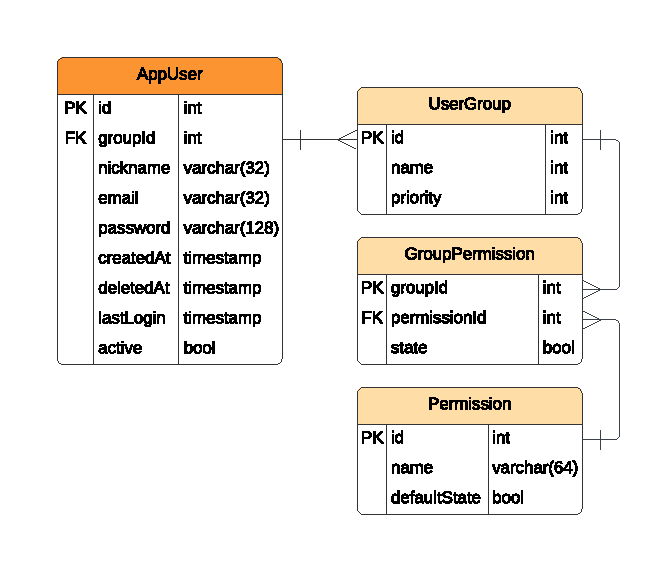
\includegraphics[width=0.7\textwidth]{diagrams/userManagement}
    \caption{Ukázka uložení uživatele v databázi. \cite{responsive_design}}
    \label{fig:user-management}
\end{figure}

\subsection{Správa obsahu}
\label{subsec:admin-elements-content-management}
Jako u správy uživatelů, správa obsahu z anglického jazyka \textit{\textquote{Content Management}} je dalším a hlavním pilířem administrativních rozhraní. Tento prvek tak umožňuje výše zmíněným rolím vytvářet, upravovat a odstraňovat obsah tak, že není nutné jakkoliv zasahovat do kódu aplikace nebo měnit čisté data ručně v databázi. Tento prvek je zásadní pro dynamické webové stránky, e-commerce platformy, blogy a další aplikace, které pravidelně mění svůj obsah nebo provádí jejich další vývoj.

Editace obsahu v aplikacích se provádí pomocí interaktivních editorů, které jsou součástí formulářů. Takové editory se nazývají WYSIWYG z anglického \textit{\textquote{What You See Is What You Get}}, tyto editory tak umožňují uživatelům editovat obsah aniž by museli znát HTML nebo CSS. Tento způsob editace je velmi oblíbený pro svou jednoduchost a přehlednost, která umožňuje i méně zkušeným uživatelům editovat obsah bez jakýchkoliv problémů. Mezi tyto populární editory patří CKEditor\footnote[1]{\url{https://ckeditor.com/}}, TinyMC\footnote[2]{\url{https://www.tiny.cloud/}} nebo Quill\footnote[3]{\url{https://quilljs.com/}}.

\subsection{Nastavení}
\label{subsec:admin-elements-settings}
Sekce pro nastavení se nachází v každém administrativním rozhraní a umožňuje tak administrátorům přizpůsobovat aplikaci podle specifických potřeb a preferencí. To může zahrnovat širokou škálu možností začínající od změny barvy, jazyka, loga, až po pokročilé možnosti jako je změna způsobu zabezpečení, různé integrace třetích stran a časté upravování SEO nastavení, které zlepšuje viditelnost aplikace ve vyhledávačích.

\subsection{Statistiky}
\label{subsec:admin-elements-statistics}
Statistiky poskytují ucelený přehled o využití a výkonost aplikace. Kde se zaměřuje na analýzu návštěvnosti, sledování chování uživatelů nebo sledování výkonu aplikace. Tento prvek tak umožňuje administrátorům sledovat aktuální stav aplikace a provádět potřebné úpravy pro zlepšení výkonu nebo zvýšení návštěvnosti.
Tyto statistiky se většinou zobrazují v podobě grafů, tabulek nebo zpráv, které poskytují uživatelům přehledné informace o aktuálním stavu aplikace.

Jako často používané nástroje pro sledování statistik se používají Google Analytics\footnote[4]{\url{https://analytics.google.com/}}, Matomo\footnote[5]{\url{https://matomo.org/}} nebo Yandex Metrica\footnote[6]{\url{https://metrica.yandex.com/}}. Při používání těchto nástrojů třetích stran je tak nutné dbát na zabezpečení a ochranu uživatelských dat, které tyto nástroje zpracovávají.

\subsection{Logování}
\label{subsec:admin-elements-logs}
Systém logování je nezbytným nástrojem pro monitorování a diagnostiku problému v aplikaci. Umožňuje tak zaznaménávat události jako jsou chyby, varování, informační zprávy nebo auditní záznamy o aktivitách uživatelů. Zpětné zobrazování těch záznamu tak pomáhá uživatelům rychle identifikovat a vyřešit problém čímž zajišťují bezpečný a nepřetržitý průběh aplikace.

\section{Administrativní značky}
\label{sec:admin-tags}
Administrativními značkami se rozumí prvky HTML, které jsou specifické pro přijímání požadavků od uživatele nebo uživateli předávají informace. Mezi takové značky patří například formuláře, tlačítka, tabulky nebo grafy. Jednotlivé značky se v nižších podkapitolách pokusím blíže přiblížit.

\subsection{Menu}
\label{subsec:admin-tags-menu}
Menu je zásadním navigačním prvkem v jakémkoliv rozhraní, umožňující uživatelů snadný přístup k rozdílným částem aplikace. Tento prvek se tak často nachází v horní částí aplikace nebo v její levé části a obsahuje tak odkazy na podřadné stránky. Důležitá je efektivnost navržení menu, kde se klade důraz na uživatelskou přívětivost a rychlou orientaci. Při velkém a rozsáhlém stromu menu tak v opačném případě dochází k častému zmatení uživatele, který pak často stránku opouští.

\subsection{Formulář}
\label{subsec:admin-tags-form}
Formuláře jsou klíčové pro interakci s uživatelem, neboť umožňují aplikaci přijímat datový vstup od uživatelů. Častým výskytem formulářů v administrativních rozhraních jsou stránky určené pro přihlášení, registraci, zadávání nebo úpravu dat. Formuláře se tak skládají z prvků jako jsou textová pole, výběrové seznamy, zaškrtávací políčka nebo obyčejné tlačítka pro provádění akce. U každého formuláře je tak důležité zabezpečení vstupu proti různým útokům, které dále budou popsány v sekci~\ref{sec:security}.

\subsection{Tlačítko}
\label{subsec:admin-tags-button}
Tlačítka jsou základním interaktivním prvkem, který umožňuje uživatelům provádět předem definované akce jako je například odeslání formuláře, potvrzení akce nebo přechod na jinou stránku. V ideálním případě by tak všechna tlačítka měla být navržena tak, aby byla pro uživatele snadno rozpoznatelná a měla tak jasně definovanou funkci. Tlačítka se tak často využívají v kombinaci s formuláři, tabulkami nebo odkazy v menu.

\subsection{Tabulka}
\label{subsec:admin-tags-table}
Tabulky jsou nezbytné pro zobrazení a přehlednou organizaci dat v strukturované formě. V administrativních rozhraních se tak tabulky využívají k zobrazení malého i velkého množství dat, například tak k zobrazení seznamu uživatelů, záznamu nebo třeba i statistikám. K tabulkám se pak vážou i často využívané prvky jako je možnost řazení, filtrování a stránkování záznamu což je nezbytné k správě velkého množství dat.

\subsection{Graf}
\label{subsec:admin-tags-chart}
Grafy nebo diagramy jsou významným prvkem pro vizualizaci dat, která se vyskytují většinou u komerčních administrativních rozhraní více než u rozhraní, které se čistě zaměřují na správu obsahu. Tyto grafy nám tak pomáhají lépe pochopit vztahy mezi data a čistě tak rozlišit vzory nebo trendy. Grafy se tak využívají pro zobrazení statistik, vývoje, analytiky a dalších měřitelných dat.

\subsection{Modální okno}
\label{subsec:admin-tags-modal}
Modální okna jsou interaktivní dialogové okna, které přitahují pozornost uživatele tak aby vykonal určitý úkon před tím, než bude moci pokračovat dále v předchozím úkonu. Tyto okna se tak často využívají pro potvrzení akce, zobrazení upozornění nebo detailního zobrazení obsahu. Jejich správné využití tak mnohem zlepšuje uživatelskou přívětivost tím, že umožní uživateli rychle reagovat bez nutnosti opustit aktuální kontext úkonu.

\section{Zabezpečení}
\label{sec:security}
Zabezpečení v rozhraních je dalším z mnoha důležitých aspektu neli ten nejdůležitější neboť se zde setkáváme s citlivými daty, které by při odcizení mohlo mít nemalý dopad na uživatele nebo samotnou aplikace. Zabezpečení se tak dělí na několik oblastí, kde každý z nich má své specifické praktiky a techniky, které zvyšují bezpečnost aplikace. V dnešní době existuje mnoho způsobu, jakým lze na danou aplikaci nebo uživatele útočit, mezi jedny z nejčastější patří \textit{SQL Injection}, \textit{Cross-Site Scripting} nebo \textit{Cross-Site Request Forgery}. V následujících podkapitolách se tak zaměřím na tyto jednotlivé oblasti.

\subsection{Autentizace}
\label{subsec:security-authentication}
Autentizace je proces, kde dochází k ověřování identity uživatele při vstupu do systému. Jedná se tak o první krok, který systém provádí před tím, než uživatel může dále interagovat s aplikací. Autentizace se tak dělí na několik základních metod, jako je přístup s \textit{uživatelským jménem a heslem}, \textit{tokenem}, \textit{biometrickými údaji} nebo \textit{certifikáty}. Každá z těchto metod má své výhody a nevýhody, které se tak většinou volí dle potřeb aplikace nebo uživatele.

Jako druhy ošetření autentizace se využívá praktik:
\begin{itemize}
    \item \textbf{Silná hesla} -- Uživatel je donucen používat heslo, které spadá do nastavené politiky administrátorem systému. Nejčastěji tak hesla musí kombinovat velká a malá písmena, čísla a speciální znaky, kde celkově heslo musí dosahovat minimálně délky 8 znaků.
    \item \textbf{Dvoufaktorová autentizace} -- Jedná se druhou vrstvu zabezpečení, kde po obyčejném přihlášení uživatele do systému, je vyžadován druhý faktor ověření. Tento faktor může být například SMS zpráva, e-mail nebo digitální token, který uživatel musí zadat pro dokončení přihlášení.
    \item \textbf{Omezení počtu pokusů} -- Tato prevence se zaměřuje na takzvaný útok hrubou sílou z anglického jazyka \textit{\textquote{Brute Force}}, kde se útočník pokouší proniknou za pomocí slovníku hesel, ale je zablokován po několika neúspěšných pokusech.
\end{itemize}

\subsection{Autorizace}
\label{subsec:security-authorization}
Autorizace se zaměřuje na rozřazení uživatelů do skupin nebo rolí, kde ověřují, zda uživatel má oprávnění provádět danou akci v systému. Nejlepším princem je tak tzv. \textit{Princip nejmenších oprávnění}, který říká, že uživatel by měl mít pouze ta oprávnění, která potřebuje pro vykonání své práce a nic víc. Často tak oprávněni uživatelé dostávají vyšší oprávnění pouze dočasně po dobu své práce a poté jsou oprávnění zpět odebrány.

\subsection{Šifrování}
\label{subsec:security-encryption}
Šifrování je procesem konverze dat do formátu, který není čitelný bez dešifrovacího klíče. Tento proces se tak často využívá u důležitých citlivých údajů jako jsou například adresy, hesla nebo platební údaje. Šifrování se tak dělí na několik základních metod, jako je \textit{symetrické šifrování}, \textit{asymetrické šifrování} nebo \textit{hashování}. Při výběru metody šifrování je tak důležité zvolit takovou metodu, která je dostatečně bezpečná a zároveň efektivní. Pro zachování zabezpečení komunikace se tak používá webový protokol HTTPS, který šifruje data za nás.

\subsection{Zabezpečení formulářů}
\label{subsec:security-forms}
Zabezpečení formulářů je klíčových prvkem pro ošetření vstupu dat od uživatele. Uživatel neboli útočník se v tomto případě pokouší o vložení škodlivého kódu do formuláře, který může mít za následek přeskočení přihlášovacích údaju, získání citlivých informací nebo zneužití aplikace. Pro ošetření formulářů se tak využívají techniky jako je \textit{validace}, \textit{filtraci} nebo \textit{escapování}.

\subsection{Zabezpečení proti útokům}
\label{subsec:security-attacks}
V moderních době počítačů existuje mnoho možnosti, jak útočnicí se mohou pokoušet proniknout do aplikace. Mezi nejčastější útoky patří \textit{SQL Injection}, \textit{Cross-Site Scripting}, \textit{Cross-Site Request Forgery} nebo \textit{Session Hijacking}. Tyto útoky se tak zaměřují na různé části aplikace, kde se snaží získat citlivé informace, zneužít aplikaci nebo získat kontrolu nad uživatelem. Pro ošetření je tak nutné implementovat několik zabezpečovacích vrstev, které tak eliminují riziko útoků.

\subsubsection*{SQL Injection}
\label{subsubsec:security-attacks-sql-injection}
SQL Injection je druh útoků, kde ůtočník vkládá neboli "injektuje" škodlivý SQL kód do vstupu formuláře, který je poté zpracováván databázovém systémem. Pokud nedojde k ošetření vstupu, útočník tak může docílit k neautorizovanému přístupu k databázi, získání citlivých informací nebo dokonce k úplnému smazání databáze.

\textbf{Obrana:} Použitím parametrizovaných dotazů, kde dochází k bezpečnému vložení dat uživatele do SQL kódu. Dále je možné omezit přístupová oprávnění uživatele databáze na minimum.

\subsubsection*{Cross-Site Scripting}
\label{subsubsec:security-attacks-cross-site-scripting}
Cross-Site scripting je dalším z druhů útoku, kde útočník podobně jako u \textit{SQL Injection} vkládá do formuláře škodlivý kód. Zde se zde ale nejedná o kód SQL ale o kód JavaScriptu. Tento kód tak může v pozadí nenápadně provádět akce, které můžou vést k odcizení cookies nebo session tokenů.

\textbf{Obrana:} Sanitace všech uživatelských vstupů. Úplné odebrání HTML značek z vstupních dat.

\subsubsection*{Cross-Site Request Forgery}
\label{subsubsec:security-attacks-cross-site-request-forgery}
Cross-Site Request Forgery je útok, pri kterém útočník využívá fakt, že daný uživatel je již autorizovaný na dané stránce. Uživatel tak po otevření odkazu je přesměrován na cílovou stránku, kde se provede nežádaná akce pod účtem uživatele.

\textbf{Obrana:} Implementace CSRF tokenu v formuláři, který zajišťuje, že požadavek přichází od správného uživatele.

\subsubsection*{Session hijacking}
\label{subsubsec:security-attacks-session-hijacking}
Session hijacking se váže na \textit{Cross-Site Scripting}, kde útočník již obdržel uživatelovu session a může tak provádět akce pod uživatelským účtem aniž by se musel sám přihlásit.

\textbf{Obrana:} Použití HTTPS protokolu, který šifruje data. Omezení platnosti session tokenů, použití dvoufaktorové autentizace a nastavení správných cookie atributů.
\newline

Každý z těchto výše zmíněných útoků představuje vážnou hrozbu pro bezpečnost aplikace a její uživatele. Proto je tak nutné dbát na správné zabezpečení aplikace a v pravidelných intervalech provádět bezpečností opatření, tak aby došlo k minimalizaci rizika útoků.

\endinput

\chapter{Použité technologie}
\label{ch:technology}
V této kapitole se budu věnovat popisu technologii, které jsem použil při vývoji rozhraní nebo jsem mezi nimi uvažoval. V první části se zaměřím na programovací jazyky, které jsou hlavní kamenem pro volbu správného frameworku. Od použití frameworku se již odvíjí další technologie spadající do kategorie frontendu a backendu. Jako poslední budu popisovat technologie, které se užívají v běžném vývoji webových aplikací.

\section{Programovací Jazyky}
\label{sec:languages}
Programovací jazyky v kontextu uživatelského rozhraní (UI) hrají klíčovou roli ve vývoji a implementaci interaktivních prvků. Proto se v této sekci zaměřím na jejich popis a konkrétní využití v rámci frameworku. Budu

Programovací jazyky a jejich správný výběr je klíčem k úspěšnému softwarovému projektu. V této sekci se pokusím popsat rozdíly mezi jednotlivými jazyky v kontextu vývoje webových aplikací a jejich využití v rámci frameworku.

\subsection{Kompilované Jazyky}
\label{subsec:languages-compiled}
Mezi první druh programovacích jazyků patří jazyky kompilované, které se při jejich zpracování převádí přímo na kód strojový. Tento proces se nazývá kompilace a výsledný kód je následně spustitelný na konkrétním operačním systému. Tento způsob zpracování má několik výhod:

\begin{itemize}
    \item \textbf{Rychlost:} Kód, který již byl jednou přeložen, je okamžitě spustitelný bez dalšího zpracování.
    \item \textbf{Výkon:} Díky překladu do strojového kódu, je možné při kompilaci provádět optimalizace, které zvyšují výkon aplikace.
    \item \textbf{Bezpečnost:} Kompilované jazyky ošetřují mnoho chyb již při jejich kompilaci, což zvyšuje bezpečnost aplikace a snižuje rizika chyb.
\end{itemize}

Mezi nejznámější kompilované jazyky můžeme zařadit jazyky jako C, C++, Java, Rust, Go a mnoho dalších. V rámci této práce jsem se zaměřil na jazyk \textit{TypeScript} a \textit{Less}, který mi tak usnadní vývoj frontendu aplikace.

\subsubsection{TypeScript}
\label{subsubsec:languages-compiled-typescript}
TypeScript je jedním z kompilovaných jazyků, který byl vytvořen jako nadstavba nad existující jazyk \textit{JavaScript}. Poprvé bych uveden v roce 2012 společností Microsoft a jeho hlavním cílem je obohacení JavaScriptu o statické typování, které umožňuje programátorům definovat typy proměnných, parametrů funkci a návratových hodnot. Mimo statické typování dále obohacuje JavaScript o funkce jako jsou třídy, moduly, generické typy a další. Díky těmto funkcím je možné zabezpečit kód proti chybám, které by mohli vzniknout v průběhu vývoje aplikace pod standardním JavaScriptem.

Oproti jiným jazykům sám o sobě není spustitelný, ale je nutné jej nejprvě přeložit do kódu JavaScriptu, Tento proces se nazývá transpilace pomocí nástroje \textit{tsc}, který je součástí balíčku \textit{Node.js}.

\subsubsection{Less}
\label{subsubsec:languages-compiled-less}
Less je dalším z kompilovaných jazyků, které se zaměřují na zlepšení a obohacení jazyka \textit{CSS}. Tento jazyk byl vytvořen v roce 2009 autorem Alexis Sellier a jako TypeScript je jeho cílem poskytnout dodatečné funkce pro pohodlnější a efektivnější psaní kaskádových stylů. Jako hlavní výhody můžeme uvést možnost definovat proměnné, funkce nebo vnořování selectoru.

Pro využití Less je nutné jej přeložit do kódu CSS, což je možné provést pomocí nástrojů jako jsou \textit{Less.js} nebo \textit{Node.js}.

\subsection{Interpretované Jazyky}
\label{subsec:languages-interpreted}
% TODO: about

\subsubsection{JavaScript}
\label{subsubsec:languages-interpreted-javascript}
% TODO: What is JavaScript

\subsubsection{Python}
\label{subsubsec:languages-interpreted-python}
% TODO: What is Python

\subsection{Značkovací Jazyky}
\label{subsec:languages-markup}
% TODO: about

\subsubsection{HTML}
\label{subsubsec:languages-markup-html}
% TODO: What is HTML

\subsubsection{Markdown}
\label{subsubsec:languages-markup-markdown}
% TODO: What is Markdown

\section{Frameworky}
\label{sec:dev-framework}
Framework, v jiných slovech struktura nebo kostra, představuje v informatice a softwarovém inženýrství abstraktní koncept poskytující základní stavební kameny pro aplikace s širokým spektrem funkcí. Cílem frameworků je usnadnit vývoj aplikací tím, že nabízejí předem definovanou strukturu, kterou lze dále rozšiřovat o vlastní kód a funkcionalitu. Tímto způsobem umožňují frameworky vývojářům rychleji a efektivněji vytvářet aplikace, což přináší zvýšení produktivity, snížení nákladů na vývoj a hlavně standardizaci kódu mezi vývojáři.

Ve svéře informatiky se frameworky dělí podle programovacího jazyku nebo zaměření na aplikace. Máme zde druhy frameworku určených na vývoj webů, her, mobilních aplikací nebo čistě na široký výzkum. \cite{about_framework}

\subsection*{Rozdíl mezi Frameworkem a Knihovnou}
Framework a knihovna jsou dvě často zaměňované koncepce, avšak existují zásadní rozdíly mezi nimi. Knihovna je soubor funkcí nebo tříd, které lze využít při vytváření aplikace. Zajišťuje určitou funkcionalitu, ale vývojář nese odpovědnost za řízení toku aplikace a volání funkcí knihovny.

Naopak framework poskytuje kompletní strukturu aplikace, kde vývojář implementuje pouze specifickou funkcionalitu. Framework tak aktivně řídí tok aplikace a volá konkrétní části kódu, zatímco vývojář se zaměřuje na přizpůsobení těchto specifických částí.

\begin{figure}[H]
    \centering
    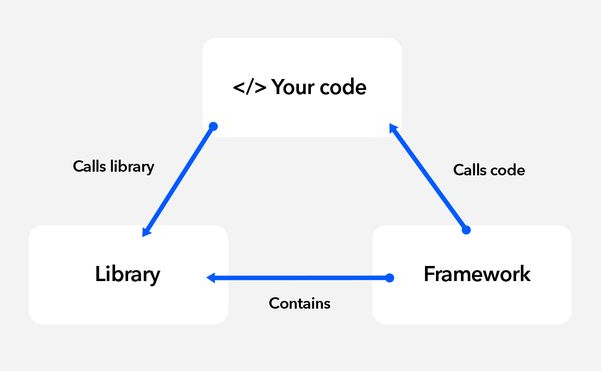
\includegraphics[width=0.6\textwidth]{figures/framework_library_difference}
    \caption{Rozdíl mezi \textit{Frameworkem} a \textit{Knihovnou}. \cite{framework_library_difference}}
    \label{fig:framework_library_difference}
\end{figure}

\subsection*{Model-View-Template vs. Model-View-Controller}
Model-View-Template dále jen jako MVT a Model-View-Controller dále jen jako MVC jsou návrhové vzory, které se široce využívají v softwarovém vývoji webových aplikací. Tyto vzory rozdělují průběh aplikaci do tří propojených částí, kde každá část má svou specifickou roli a odpovědnost. Díky této struktuře je možné izolovat různé části aplikace a tím zvyšovat modularitu, znovu použitelnost a udržitelnost kódu.

V případě MVT je aplikace rozdělena na tři části: \textit{Model}, \textit{View} a \textit{Template}. Model zde reprezentuje datovou strukturu, většinou tedy namapované objekty získané z databáze, případně z jiného zdroje. View (zobrazení) je zodpovědné za přijímání uživatelských požadavků a zobrazování odpovědi od serveru zpět uživateli, v rámci této komunikace reprezentuje určitý most mezi modelem a šablonou. Jako poslední je zde template (šablona), která v tomto případě přijatá data zpracovává do výsledného HTML kódu pomocí speciálních značek určující předem daný formát stránky. Výsledný HTML kód je následně odeslán zpět uživateli.

Na druhé straně MVC, který je často používán ve zbytku frameworku se oproti MVT liší pouze lehce. Model zde stále reprezentuje datovou strukturu, ale View je naopak zodpovědný o pouhé vykreslování dat uživateli. Novým prvkem je zde Controller, který se zaobírá zbylou interakcí uživatele s aplikací, tedy přijímání požadavků, zpracování dat a následné odeslání zpět uživateli. \cite{mvc_mvt_difference}

\begin{figure}[H]
    \centering
    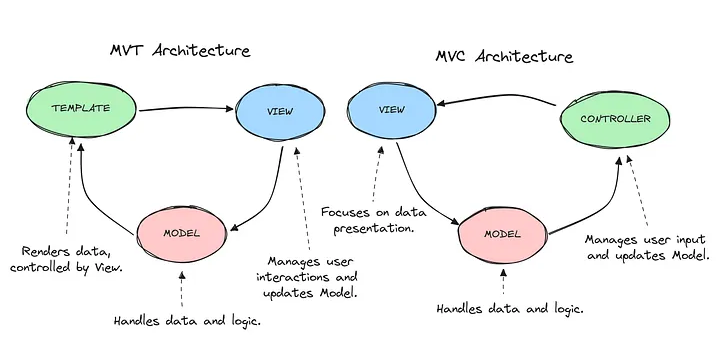
\includegraphics[width=1.0\textwidth]{figures/mvc_mvt_difference}
    \caption{Rozdíl mezi \textit{Model View Template} a \textit{Model View Controller} návrhovými vzory. \cite{mvc_mvt_difference_img}}
    \label{fig:mvc_mvt_difference}
\end{figure}

\subsection{Django}
\label{subsec:dev-framework-django}
Django je výkonným open-source frameworkem určeným pro vývoj robustních a lehce škálovatelných webových aplikací v programovacím jazyce Python. Od svého veřejného uvedení v roce 2005, pojmenovaného po slavném kytaristovi Django Reinhardtovi, získal popularitu díky své schopnosti urychlit vývoj a poskytnout bezpečné a efektivní nástroje pro tvorbu webových aplikací.

Framework Django přistupuje k architektuře webových aplikací pomocí návrhového vzoru Model-View-Template (MVT), což představuje alternativu k tradičnímu přístupu Model-View-Controller (MVC). Tato struktura usnadňuje komunikaci mezi datovým modelem, prezentační vrstvou a šablonami pro serverové vykreslování.

V oblasti vývoje uživatelského rozhraní Django nabízí šablonovací jazyk (DTL), který umožňuje vytvářet dynamická a daty řízená uživatelská rozhraní. To je zvláště užitečné pro aplikace, které kladou důraz na optimalizaci pro vyhledávače (SEO) a vyžadují komplexní logiku na straně serveru. DTL umožňuje vývojářům vytvářet stránky s dynamickým obsahem, který je generován ještě před odesláním HTML kódu ze serveru.

V situacích, kde je potřeba dosáhnout interaktivity uživatele s rozhraním, je možné rozšířit Django o JavaScriptové knihovny nebo volit jiný framework specializovaný na frontendový vývoj. To umožňuje vysoce flexibilní přístup k vytváření moderních a interaktivních webových aplikací. \cite{about_django}.

\subsection{React}
\label{subsec:dev-framework-react}
React je významná JavaScriptová knihovna určená pro vytváření uživatelských rozhraní, především na straně klienta. Vyvinutá firmou Facebook, React využívá virtuální DOM k efektivní aktualizaci komponent a podporuje deklarativní syntaxi pro tvorbu interaktivních uživatelských rozhraní. Je široce používán pro vývoj jednostránkových aplikací (SPA), kde je klíčová potřeba dynamických aktualizací.

React vyniká v poskytování responzivního a interaktivního uživatelského přístupu, což z něj činí oblíbenou volbu pro moderní webový vývoj. Jeho komponentový přístup umožňuje rozdělit uživatelské rozhraní do znovupoužitelných částí, což zjednodušuje správu a údržbu kódu. Využívá návrhový vzor \textit{Model-View-Controller}. \cite{about_react}

\subsection{Angular}
\label{subsec:dev-framework-angular}
Angular je populární open-source framework pro vývoj webových aplikací. Je sponzorován a udržován převážně společností Google a vyniká díky široké komunitě a schopnosti řešit výzvy spojené s vývojem jednostránkových aplikací (SPA). Angular je postaven na jazyce TypeScript a využívá komponentovou architekturu pro tvorbu uživatelských rozhraní.

Jednou z klíčových vlastností Angularu je jeho komplexní systém modulů a komponent, který usnadňuje organizaci a správu kódu. Angular používá návrhový vzor \textit{Model-View-Controller} (MVC) a klade důraz na dvoucestný data-binding, což znamená, že změny v modelu automaticky odrážejí změny v vykreslování a naopak.

Framework obsahuje mnoho vestavěných funkcí, jako například modulární routování, HTTP služby pro komunikaci se serverem, a nástroje pro testování. Angular také poskytuje kompletní sadu nástrojů pro správu stavu aplikace. \cite{about_angular}

\subsection{Laravel}
\label{subsec:dev-framework-laravel}
Laravel je moderní open-source PHP framework, který je určený pro vývoj webových aplikací. Tento framework vytvořil Taylor Otwell a byl poprvé vydán v roce 2011. Vyniká díky své jednoduchosti, efektivitě a schopnosti urychlit vývoj aplikací. Laravel využívá návrhový vzor \textit{Model-View-Controller} (MVC) a poskytuje mnoho vestavěných funkcí, jako například routování, šablonovací systém, a nástroje pro správu databáze.

Mezi jednu z jeho klíčových vlastností patří Eloquent ORM, což je moderní implementace Active Record návrhového vzoru, který umožnuje jednoduše pracovat s namapovanými objekty z databáze jako s obyčejnými PHP objekty. Jako framework Django obsahuje šablonovací systém Blade, které je jednoduchý a efektivní pro vytváření dynamických uživatelských rozhraní. Další výhodou jsou zabudované mechanismy pro zabezpečení aplikace, jako například ochrana proti Cross-Site Scripting (XSS) a SQL Injection útokům. \cite{about_laravel}

\subsection{Vue.js}
\label{subsec:dev-framework-vuejs}
Vue.js je moderní JavaScriptový framework určený pro vývoj uživatelského rozhraní webových aplikací. Jeho největší výhodou je snadná flexibilita a jednoduchá intergrace s již existujícími projekty. Vue.js byl poprvé vydán v roce 2014 a od této doby získal velkou popularitu díky své schopnosti urychlit vývoj a poskytnout efektivní nástroje pro tvorbu moderních webových aplikací.

Jedním z klíčových prvků Vue.js je reaktivní datová vrstva, která umožňuje snadná sledování a aktualizaci dat. Framework využívá jednosměrný datový tok, což znamená, že veškeré změny v datech jsou automaticky aktualizovány v uživatelským rozhraní. Toto chování usnadňuje sledování stavu aplikace a vytváření dynamických a interaktivních uživatelských rozhraní.

Vue.js je navržen ohledem na progresivitu, což znamená, že ho lze snadno a postupně intergrovat do existujícího projektu a nijak tak nenarušit jakoukoliv funkčnost. Při této integraci lze jednoduše rozdělit aplikaci do Frontend části, reprezentovanou Vue.js a backend části, která může být reprezentována například frameworkem Django. \cite{about_vuejs}

\subsection{Svelte}
\label{subsec:dev-framework-svelte}
Svelte je jedním z inovativních JavaScriptových frameworků, který se zaměřuje na efektivní kompilací v ranné fázi build procesu, což přináší nový pohled na vývoj uživatelské rozhraní. Zatímco tradiční frameworky provadějí většinu práce na straně klienta nebo serveru za běhu, Svelte přesouvá tuto činnost do fáze komiplace, čímž mnohonásobně zlepšuje výkon a optimalizuje výslednou velikost kódu.

Klíčovým konceptem Svelte je štěpení kódu do komponent, které jsou více než pouze části uživatelské rozhraní. Tyto komponenty obsahuje více než prezentační logiku, definují také jak se má komponent chovat a jaké akce má provádět pod určitými podmínkami. Tento přístup tak umožnuje jednoduše eliminovat zbytečný nebo duplicitní kód ve fázi kompilace, jako dělají například \textit{C++ kompilátory}.

Pro plné využití tohoto frameworku, je nutné jeho rozšíření o backendovou část, která bývá zodpovědná za zpracování dat a komunikaci se serverem. Tato část může být reprezentována například jedním s frameworků zmíněných výše. \cite{about_svelte}

\subsection{Shrnutí a Srovnání}
\label{subsec:dev-framework-comparison}
Srovnání frameworku zmíněných výše dosahuje celkového závěru, že každý z ních má své výhody a nevýhody. Pomocí každého frameworku nebo jejich kombinací lze vytvořit moderní a efektivní webové aplikace, které by splňovaly mnoho požadavků ze strany efektivního vývoje, výkonu a bezpečnosti.
Každý z frameworků používá jiný jazyk, ať to je buď Python, JavaScript nebo PHP, což může být klíčové pro jeho výběr vzhledem k projektu. Dalším faktorem je dokumentace, komunita a dostupnost nástrojů, které mohou zajistit rychlý vývoj a řešení problémů.

Pro můj projekt jsem nakonec zvolil \textbf{Django}. Tento framework jsem zvolil z důvodu, že jsem s ním již v minulosti pracoval a mám tedy určité znalosti a schopnosti pracovat pod jazykem Python. Pokud se podíváme na srovnání frameworku, Django není moc populárním v oblasti frontendu, ale díky jeho šablonovacímu systému a možností rozšíření o JavaScriptové knihovny lze tyto nedostatky vykompenzovat.

\begin{figure}[H]
    \centering
    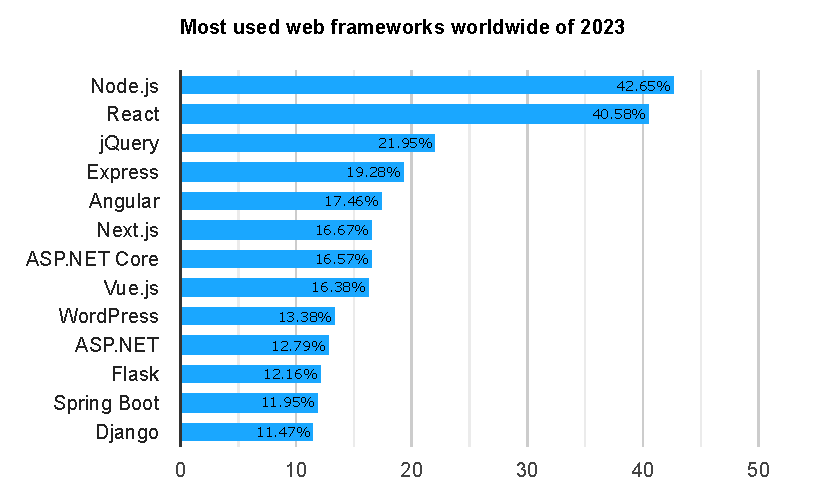
\includegraphics{figures/frameworkGraphs}
    \caption{Srovnání webových frameworku pro rok 2023. \cite{framework_comparison}}
    \label{fig:framework_comparison}
\end{figure}

\section{Zpracování požadavku}
\label{sec:dev-request-processing}
Zpracování požadavku je klíčovým prvkem webových aplikací, vzhledem k rozsáhlým rozdílům u frameworku je nutné si blíže představit jak takové zpracování probíhá. V rámci tohoto procesu se setkáváme s dvěma typy zpracování \textit{Server-Side} a \textit{Client-Side}. Jako třetí druh zpracování se dá považovat i \textit{Hybridní} neboli \textit{Pre-Rendering}, který kombinuje oba přístupy.

Při vývoji je nutné si předem určit, který ze stylů zpracování bude pro projekt použit, přechod mezi jednotlivými druhy již v průběhu vývoje může být velmi zdlouhavý a finančně náročný. \cite{request_processing}

\subsection{Server-Side Rendering}
\label{subsec:dev-request-processing-server-side-rendering}
Server-Side Rendering (SSR) je často využívaný způsob zpracování, který se obvykle uplatňuje u menších webových aplikací, jež bývají označovány jako statické stránky. Tyto stránky svůj obsah po zpracování již nikdy nemění. Základem SSR je, že veškeré zpracování dat probíhá na straně serveru, a klient poté již obdrží kompletně vykreslenou stránku, kterou prohlížeč jednoduše načte. Tyto stránky díky své statické povaze dosahuji často vysokých hodnocení v SEO, což je klíčové pro zvýšení návštěvnosti.

Jednou z nevýhod SSR je však vysoká náročnost na vypočetní výkon serveru. Tento problém se projevuje zejména v případě, kdy server zaznamená velké množství klientských požadavků v krátkém časovém období. Při každém požadavku dojde k novému kompletnímu vykreslení stránky, i když se obsah stránky změnil jen minimálně.

\begin{figure}[H]
    \centering
    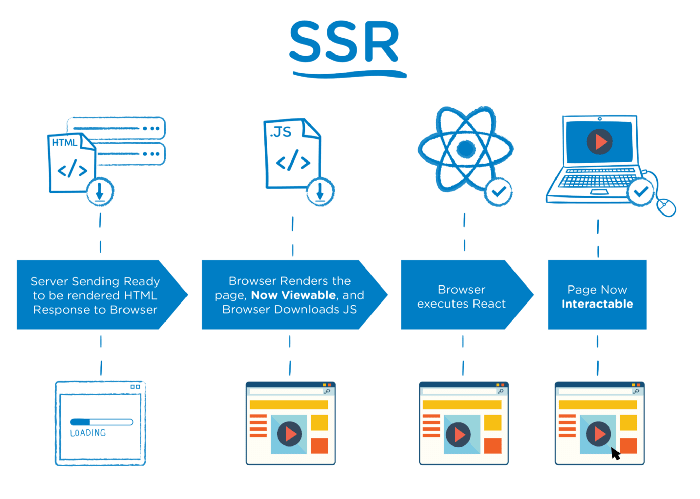
\includegraphics[width=1.0\textwidth]{figures/server-side-rendering}
    \caption{Postup Server-Side renderingu při žádosti o stránku. \cite{rendering-diff}}
    \label{fig:server-side-rendering}
\end{figure}

\subsection{Client-Side Rendering}
\label{subsec:dev-request-processing-client-side-rendering}
Client-Side Rendering (CSR) je moderní způsob zpracování webových stránek, jehož využití se rozšířilo s příchodem programovacího jazyka JavaScript do světa World-Wide-Web (WWW). Tento přístup umožňuje dynamické vykreslování obsahu stránek přímo na straně klienta, což výrazně snižuje zátěž serveru a zvyšuje rychlost zpracování požadavků.

Ve srovnání s Server-Side Renderingem (SSR) je u CSR náročnější dosáhnout vysokého skóre v oblasti SEO. Důvodem je, že proces vykreslování stránky u klienta může trvat proměnlivě dlouho a existují rizika, že webcrawler, který indexuje stránku ji opustí ještě před jejím kompletním načtením. Tento problém lze řešit pomocí techniky \textit{Pre-Rendering}, kterou popisuji v následující sekci.

\begin{figure}[H]
    \centering
    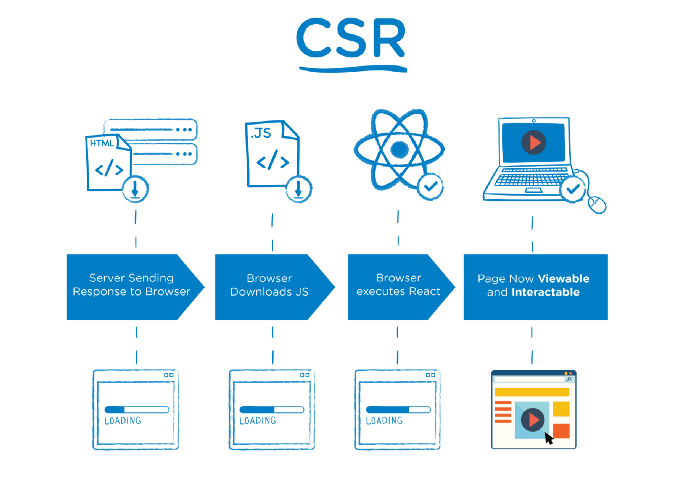
\includegraphics[width=1.0\textwidth]{figures/client-side-rendering}
    \caption{Postup Client-Side renderingu při žádosti o stránku. \cite{rendering-diff}}
    \label{fig:client-side-rendering}
\end{figure}

\subsection{Hybrid Rendering}
\label{subsec:dev-request-processing-hybrid-rendering}
Hybrid Rendering, také známy jako Pre-Rendering, představuje moderní přístup k zpracování webových stránek, který se pokouší o skloubení výhod Server-Side a Client-Sider renderingu. Tento přístup jednoduše umožnuje vývojářům vytvářet takhzvané "skeleton" stránky, které jsou odeslány klientovi ihned po přijetí požadavku. Po následném načtení stránky klientem, dochází k dynamickému vykreslení obsahu, kde dojde k nahrazení pouze daných části webu, které obsahovaly dynamický obsah.

\section{Technologie}
\label{sec:dev-technology}
V nynější sekci se zaměřím na popis bližší popis technologii, které lze využívat během vývoj nebo přímo v rámci daného frameworku. Mezi tyto technologie spadá široké spektrum nástrojů, knihoven, jazyký a dalších prvků, které jsou volně dostupné na internetu a mají za cíl usnadnit vývoj a zvýšit efektivitu vývojáře.

\subsection{Šablonování}
\label{subsec:dev-technology-templating}
Šablonování je klíčovou technologií v rámci vývoje webových aplikací, která slouží k oddělení prezentace dat od logiky jejich zpracování. Tento přístup umožňuje vývojářům a designérům efektivně spolupracovat na vytváření jak statických tak dynamických uživatelských rozhraní, zatímco zvyšuje modularitu, udržitelnost a bezpečnost kódu. Šablonování se většinou využívalo jako externí knihovna, ale s příchodem moderních frameworků jako je Django, React nebo Angular, se stalo nedílnou součástí těchto frameworků.

Jako systém umožňuje definovat strukturu a vzhled webových stránek pomocí šablon, které se na sebe mohou vázat nebo se rozšiřovat. Každá z těchto šablon obsahuje statický HTML kód spolu s vloženými proměnnými, filtry a řídícími strukturami. Finální šablony se poté před odesláním klientovi zpracují na serveru, a výsledný HTML kód je odeslán klientovi.

Mezi hlavní výhody používání šablon patří:
\begin{enumerate}
    \item \textbf{Oddělení Prezentace a Logiky:} Šablonovací systém oddělením prezentace dat a logiky zpracování umožňuje vývojářům a designérům efektivně spolupracovat.
    \item \textbf{Univerzální Použitelnost:} Šablony lze použít pro vytváření jak statických tak dynamických uživatelských rozhraní, což zvyšuje modularitu a znovupoužitelnost kódu.
    \item \textbf{Podpora Dynamických Dat:} Díky použití proměnných a filtrů umožňuje šablonovací systém dynamicky zobrazovat data na stránkách. To je klíčové pro vytváření interaktivních a daty řízených uživatelských rozhraní.
    \item \textbf{Zabezpečení:} Systém frameworku obsahuje mechanismy pro prevenci útoků jako Cross-Site Scripting (XSS), Form tampering, SQL injection a další. Tato zabezpečení jsou automaticky aplikována na šablony, což zvyšuje bezpečnost aplikace.
\end{enumerate}

Celkově lze konstatovat, že technologie šablonování přispívá k efektivnímu a strukturovanému vývoji webových aplikací, usnadňuje spolupráci mezi vývojáři a designéry a zvyšuje obecnou robustnost aplikace. Pro svůj projekt jsem zvolil šablonovací systém \textbf{Django Template Language (DTL)}, který je součástí frameworku Django.
\\

% Code example
\lstinputlisting[language=HTML, caption={Příklad použití templatu v Djangu.}, label={lst:django-template-example}]{sourceCodes/DjangoTemplateExample.html}

\subsection{Balíčkovací systémy}
\label{subsec:dev-technology-package-managers}

% TODO: Možná odstranit?
\textcolor{red}{Možná odstranit? Jedná se o technologii, kterou hojně využívám, ale nevím zda je to vhodné pro tuto sekci.}

\subsubsection{NPM}
\label{subsubsec:dev-technology-package-managers-npm}

\subsubsection{Yarn}
\label{subsubsec:dev-technology-package-managers-yarn}

\subsubsection{PIP}
\label{subsubsec:dev-technology-package-managers-pip}

\subsection{Boostrap}
\label{subsec:dev-technology-bootstrap}

\endinput
\chapter{Implementace}
\label{ch:implementation}
Tato sekce obsahuje popis implementace aplikace, která byla vytvořena na základě analýzy v předchozích kapitolách. V této sekci se zaměřím na popis jednotlivých komponent aplikace, které byly vytvořeny a následně nasazeny do produkce. Dále se zaměřím na popis týmové spolupráce, která byla nutná pro vytvoření celého projektu, a na závěr se zaměřím na popis problémů, které se v průběhu vývoje objevily.

\section{Požadavky na implementaci}
\label{sec:implementation-requirements}
Požadavků na implementaci ze strany administrativního rozhraní není mnoho, přesto ale existují. V této sekci se pokusím popsat veškeré požadavky, které byly kladeny na implementaci aplikace během jejího návrhu.

Během vývoje se tyto požadavky průběžně měnily, proto je celkem obtížné vždy předem definovat úplný seznam požadavků.

\subsection*{Funkční požadavky}
\label{subsec:implementation-requirements-functional}

\begin{description}
    \item \textbf{Přihlášení} -- Jelikož se jedná o aplikaci administrační, vstup do aplikace je možný pouze pro přihlášené uživatele. Z funkčního hlediska je v rámci projektu využita pouhá role \textit{Administrátora}, z toho důvodu není nutné rozlišovat mezi různými uživatelskými rolemi.
    \item \textbf{Správa obsahu} -- Hlavním účelem tohoto rozhraní je správa obsahu hry, bez možnosti formulářové editace obsahu jsou administrátoři omezeni na surovou správu dat pomocí editace záznamů v databázi nebo změnou výchozích dat v souborech. Z tohoto důvodu je nutné zajistit plnou možnost správy obsahu hry stylem \textit{CRUD}.
    \item \textbf{Filtrace a vyhledávání} -- Pro přehlednou správu dat jednotlivých tabulek je důležité umožnit administrátorům rychlé a efektivní prvky filtrování.
    \item \textbf{Vykreslování} -- Určité části projektu obsahují grafické prvky, které je pro lepší pochopení nutné graficky zpracovat a vykreslit na obrazovku. Pro tento účel bude využit HTML prvek \textit{canvas}, který umožňuje grafické vykreslování.
    \item \textbf{Validace} -- Při vkládání obsahu do databáze pomocí API je nutné klást důraz na správné formátování všech dat před odesláním.
    \item \textbf{Export} -- Pro úspěšné zálohování dat je nutné umožnit export všech dat do souboru, který bude následně kompatibilní s automatickým importem do databáze.
\end{description}

\section{Komponenty aplikace}
\label{sec:implementation-components}
V případě implementace administračního rozhraní nelze pouze implementovat frontend aplikace, ale je nutné implementovat i backend, který zajišťuje zpracování dat, a jejich následnou komunikace s API\@.

V níže uvedených sekcích se blíže zaměřím na implementaci jednotlivých komponent.

\subsection{Frontend}
\label{subsec:implementation-frontend}
Vývoj frontendu byl zahájen vyhledáním již předem vytvořené šablony a to z důvodu usnadnění designových potřeb a možnosti se plně věnovat další části aplikace. Výsledek hledání byl úspěšný a nalezená šablona byla kompatibilní s frameworkem Django. Přesněji se jedná o šablonu od autora \textit{Themesberg}\footnote{\href{https://themesberg.com/}{https://themesberg.com/}}, konkrétně šablona administračního rozhraní \textit{Volt}\footnote{\href{https://themesberg.com/product/django/volt-admin-dashboard-template}{https://themesberg.com/product/django/volt-admin-dashboard-template}}.

Po úspěšné instalaci bylo dalším krokem rozvržení navigace, která se nachází na levé straně stránky. Jednotlivé odkazy následně směřují na podstránky, kde lze vidět obsah jednotlivých tabulek, ve kterých se nachází možnost filtrovat, hledat nebo provádět zbytek CRUD operací.

Průběh otevření každé ze stránek navigace je možné vidět na Diagramu~\ref{fig:OpenPage}, kde prvně dochází k ověření přihlášení uživatele, následnému zobrazení dočasného obsahu stránky, který je v pozdější době asynchronně doplněn obsahem z API\@.

\processDiagram{diagrams/OpenPage}{OpenPage}{0.75\textwidth}{Diagram zobrazující otevření stránky}

\subsection{Backend}
\label{subsec:implementation-backend}
Backend aplikace, vytvořen pod frameworkem Django stejně jako část frontendu, zajišťuje zpracování dat podle žádosti uživatele. K získání dotazu dochází pomocí URL adresy, která je v aplikaci zpracována pomocí \textit{view} komponenty pod následnou routing adresou. Po vyřízení požadavku jsou data zpět odeslána uživateli, který je následně upozorněn na úspěšné provedení akce.

Níže zobrazený Diagram~\ref{fig:NewObject} popisuje průběh vytvoření nebo editace objektu, kde tato funkcionalita reprezentuje nejdůležitější prvek celé aplikace z důvodu, že umožňuje definovat herní obsah. Po odeslání formuláře dochází ke kontaktování API, která následně požadavek zpracuje a odešle zpět odpověď, jež je následně zobrazena uživateli.

\processDiagram{diagrams/NewObject}{NewObject}{0.75\textwidth}{Diagram reprezentující průběh vytvoření nebo editace objektu}

\subsection{API}
\label{subsec:implementation-api}
Přestože API je součástí práce kolegy, pro usnadnění a zabezpečení jsem použil vlastní lokální API, které zpracovává dotazy, a v případě, že je nutné získat data, odešle požadovaný dotaz směrem na veřejné API pod url adresou \textit{https://api.tts-game.fun}. Díky zmíněnému mezikroku je možné zabezpečit identitu API klíče, který zůstává skrytý pod lokálním API spravovaným jazykem Python. V opačném případě by tento klíč byl odesílán s každým dotazem, čímž by se stal zachytitelný pro útočníky.

V našem případě jsme použili pro autorizaci obyčejný token, které je uložen v nastavení API. Nejedná se o nejbezpečnější použití, ale z pohledu této práce je dostatečné. Schéma komunikace při použití prostřední API je možné vidět na Obrázku~\ref{fig:api_communication}.

\begin{figure}[H]
    \centering
    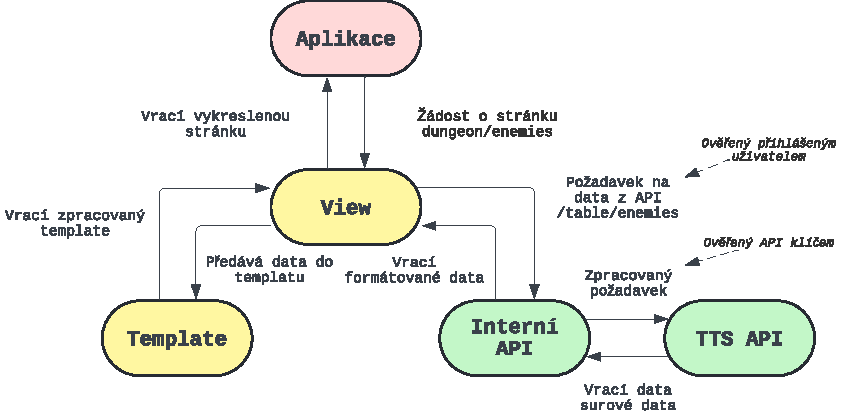
\includegraphics[width=0.96\textwidth]{diagrams/API_Communication}
    \caption{Schéma komunikace mezi jednotlivými komponentami}
    \label{fig:api_communication}
\end{figure}

\section{Volba technologií}
\label{sec:implementation-technologies}
V této sekci se budu věnovat výběru technologií, které jsem zvolil v průběhu implementace aplikace. Výběr technologií většinou vychází z analýzy uvedené v Kapitole~\ref{ch:theory_and_analysis} nebo z osobních zkušeností, které jsem získal v průběhu studia.

\subsection{Framework}
\label{subsec:implementation-technologies-framework}
Jak bylo zmíněno v sekci analýze rozhraní, pro vývoj aplikace administrativního rozhraní jsem zvolil framework Django. Díky tomuto frameworku jsem mohl využít jeho širokou škálu již předem zakomponovaných funkcí, které mi usnadnily vývoj. Díky těmto funkcím jsem se mohl zaměřit na vývoj samotného rozhraní, které jsem psal v jazyce TypeScript s využitím frontendového frameworku Bootstrap.

Framework jako samotný neobsahuje rozšířené prvky pro použití na frontendu, z toho důvodu jsem byl nucen psát si tyto komponenty sám. Pro jejich vývoj jsem využil jazyk TypeScript, kde jsou výsledné komponenty mezi stránkami sdíleny. Pro dynamické načítaní obsahu je využíváno asynchronní načítání dat pomocí AJAXu po prvotním načtení stránky a po jeho zpracování dojde k překreslení části stránky.

Jedna z komponent, která slouží pro asynchronní získávání dat je zobrazena v ukázce Zdrojového Kódu~\ref{lst:data-request-component}. Tato komponenta slouží pro nahrazení dočasného obsahu na stránce daty, která jsou získána v pozdějším procesu pomocí XMLHttpRequestu, který je volán na interní API, kde následně dochází k vyplnění obsahu templatu daty a jeho zobrazení.

\lstinputlisting[language=TypeScript, caption={Komponenta pro získání asynchronních dat}, label={lst:data-request-component}]{sourceCodes/DataRequestComponent.ts}

\subsection{Knihovny}
\label{subsec:implementation-technologies-libraries}
Při vývoji aplikace jsem využil několik knihoven třetích stran, které mi usnadnily vývoj a zároveň zrychlily proces vývoje, protože nebylo nutné psát vše od základu. Mezi tyto knihovny patří:

\begin{description}
    \item \textbf{Font Awesome}\footnote{\href{https://fontawesome.com/}{https://fontawesome.com/}} je knihovna ikon, která disponuje širokou škálou veřejně dostupných ikon, které jsou zdarma k použití. Ve vývoji jsem tyto ikony použil pro reprezentaci různých akcí, které může uživatel provést.
    \item \textbf{Bootstrap}\footnote{\href{https://getbootstrap.com/}{https://getbootstrap.com/}} jsem použil jako frontendovou knihovnu předem napsaných stylů, díky kterým jsem mohl rychle vytvořit efektivní a responzivní rozhraní. Bootstrap nabízí širokou škálu komponent, které jsou podrobně popsány v dokumentaci.
    \item \textbf{SweetAlert2}\footnote{\href{https://sweetalert2.github.io/}{https://sweetalert2.github.io/}} je knihovna, která umožňuje jednoduše zobrazovat notifikace a upozornění uživateli. Knihovna byla využita například pro zobrazení upozornění při chybě nebo úspěšném provedení akce.
    \item \textbf{GoJS}\footnote{\href{https://gojs.net/latest/index.html}{https://gojs.net/latest/index.html}} obsahuje funkce pro jednoduché a efektivní vytváření grafů, které byly využity pro interaktivní zobrazení návaznosti lokací v rámci kampaně.
    \item \textbf{Animate.css}\footnote{\href{https://animate.style/}{https://animate.style/}}, Hover.css\footnote{\href{https://ianlunn.github.io/Hover/}{https://ianlunn.github.io/Hover/}} je knihovna, která obsahuje předpřipravené animační styly, které stačí pouze aplikovat pomocí CSS tříd nebo dynamicky pomocí JavaScriptu.
    \item \textbf{Notiflix}\footnote{\href{https://notiflix.github.io/}{https://notiflix.github.io/}} je další z knihoven pro zobrazování notifikace, v tomto projektu jsem ale pro notifikace zvolil knihovnu SweetAlert2. Z toho důvodu je tato knihovna využita pouze pro blokaci uživatelského vstupu během načítání nebo zpracování dat formou loading spinneru.
    \item \textbf{NoUISlider}\footnote{\href{https://refreshless.com/nouislider/}{https://refreshless.com/nouislider/}} je knihovna, která do prvků HTML přidává možnost vytvořit posuvníky, které je následně možné využit pro výběr hodnoty z rozsahu. Příklad jeho použití je ve formuláři s filtrací dat.
\end{description}

\subsection{Jazykový procesor}
\label{subsec:implementation-technologies-compiler}
Výběr jazyka pro uživatelské rozhraní je důležitým aspektem v případě aplikací určených pro širokou veřejnost. V rámci této práce byl jako primární jazyk rozhraní zvolen jazyk anglický, což je nejuniverzálnější jazyk na světě, díky čemuž je aplikace přístupná širokému spektru uživatelů bez potřeby překladu. Nicméně pro některé uživatele může být angličtina obtížná, a z toho důvodu byl implementován jazykový procesor, který umožňuje integraci více jazyků do aplikace.

Pro podporu vícejazyčné funkčnosti byla v této práci využita knihovna i18next\footnote{\href{https://www.i18next.com/}{https://www.i18next.com/}}, která je jednou z nejrozšířenějších nástrojů pro lokalizaci. Tato knihovna automaticky zpracovává jazykové soubory a aplikuje odpovídající překlady v závislosti na nastavení uživatele. Tímto způsobem je pro vývojáře snadné nastavit výchozí jazyk a později přidat další překlady.

\lstinputlisting[language=JavaScript, caption={Ukázka využití knihovny i18next}, label={lst:i18next-example}]{sourceCodes/LanguageLocalization.js}

Na ukázce Zdrojového Kódu~\ref{lst:i18next-example} je zobrazeno využití knihovny v případě obyčejného použití v JavaScriptu. Knihovna sama o sobě nabízí možnou integraci do různých frameworků jako například použitý freamework Django v této práci.

\subsection{Databáze}
\label{subsec:implementation-technologies-database}
Pro ukládání dat v našem systému jsme zvolili databázi MariaDB\footnote{\href{https://mariadb.org/}{https://mariadb.org/}}, která nám byla doporučena vedoucím práce. Nejedná se o nejmodernější databázi, ale disponuje vysokou stabilitou a širokou historii použití. Databázi jsme pro bezpečnější použití rozdělili na dvě \textit{tts\_api} a \textit{tts\_api\_dev}, kde první obsahuje základní data a druhá data testovací. Pro vytvoření databáze byly následně využity skripty, které budou dále popsány v sekci Automatizace.

\subsubsection*{Schéma}
\label{subsubsec:implementation-technologies-database-scheme}
Schéma databáze bylo vytvořeno placeným softwarem DbDiagram.io\footnote{\href{https://dbdiagram.io/home}{https://dbdiagram.io/home}}, který nabízí možnost živého návrhu schématu, na kterém se tak mohl podílet každý člen týmu zároveň, což usnadnilo aktivní vývoj. Zkrácené schéma o M:N relacích je zobrazeno na Obrázku~\ref{fig:db_scheme}. Software DbDiagram nabízí možnost exportu schématu do různých formátů, které byly následně využity pro vytvoření databáze v MariaDB\@.

% disgusting!
\begin{figure}[H]
    \centering
    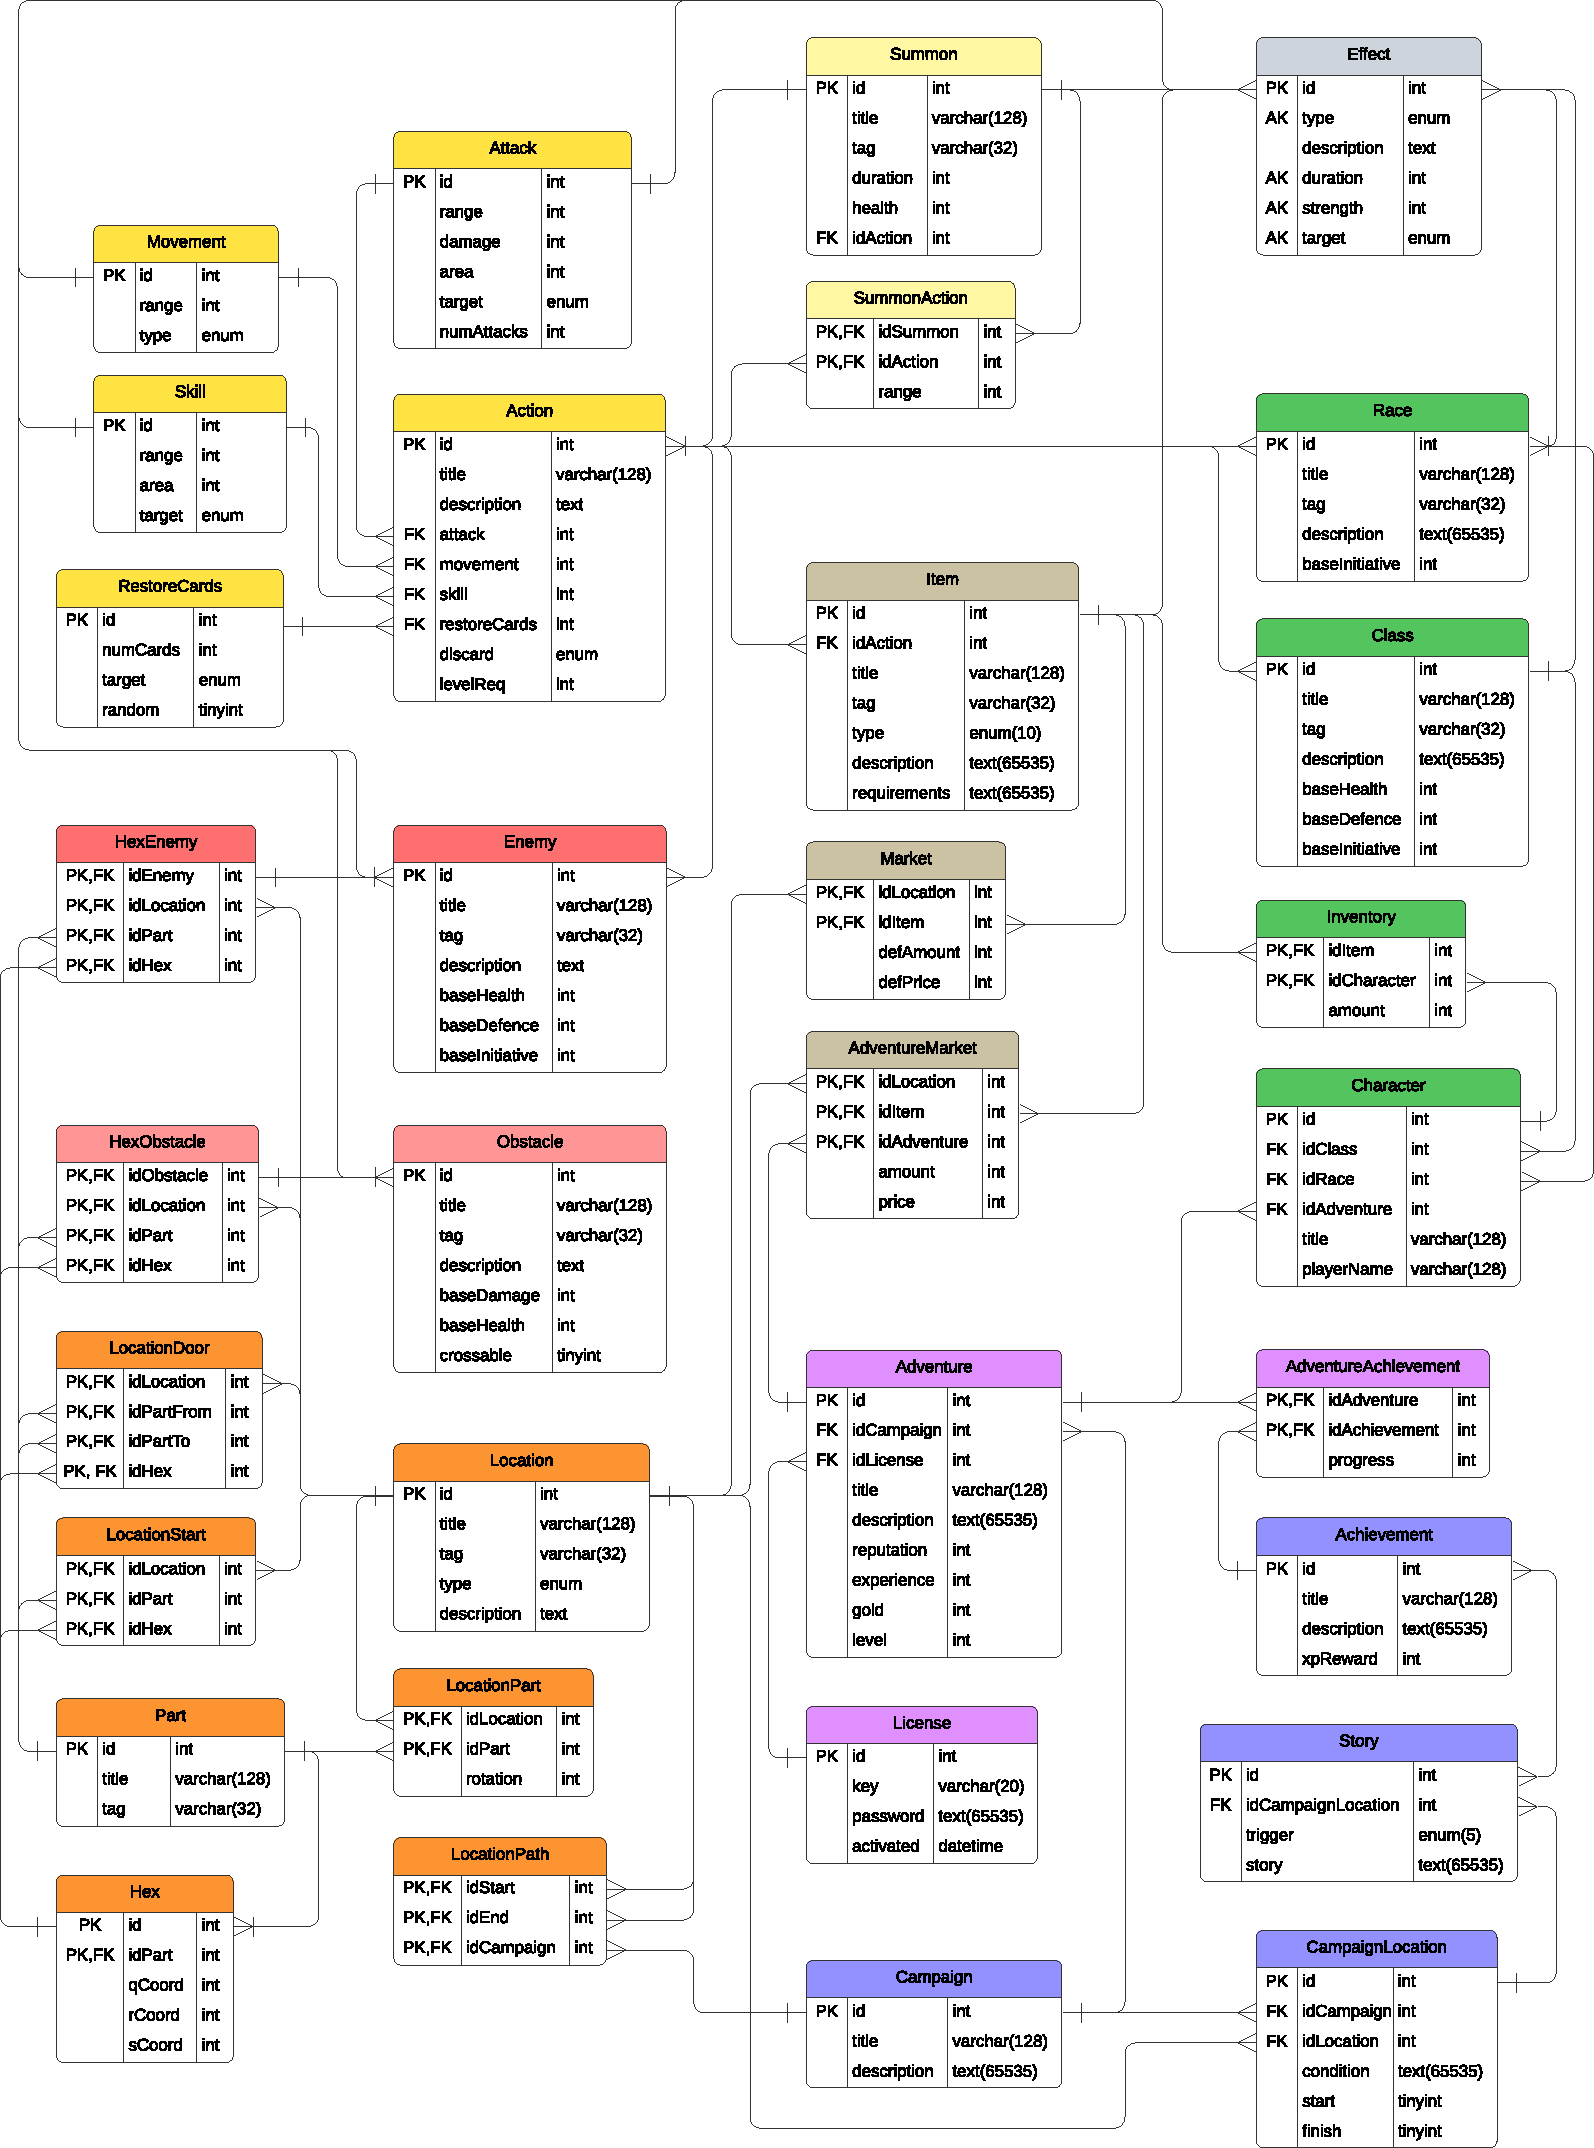
\includegraphics[width=0.96\textwidth]{../../shared/diagrams/dbScheme}
    \caption{Kompletní schéma databáze}
    \label{fig:db_scheme}
\end{figure}

\subsubsection*{Automatizace}
\label{subsubsec:implementation-technologies-database-automatization}
Automatizace vytváření a plnění databáze je důležitá pro kontinuální vývoj softwaru a v praxi se nazývá \textit{migrace}. Skripty pro vytvoření a naplnění databáze byly napsány v skriptovacím jazyce Python\footnote{\href{https://www.python.org/}{https://www.python.org/}}. Tyto skripty byly vytvořeny tak, aby při jejich spuštění provedly kompletní smazání databáze, následně pak její znovuvytvoření a pozdější naplnění. Ukázka výstupu vytvořených skriptů je zobrazena v příloze~\ref{fig:databaseScriptsOutput}.

Pro vytvoření databáze byl použit SQL soubor, který se po každé úpravě v nástroji DbDiagram.io vyexportoval. Jakmile byla databáze resetována do výchozí podoby a vše proběhlo úspěšně, došlo na řadu její plnění, pro které jsou data uložena v souborech ve formátu JSON. Tyto soubory lze jednoduše exportovat z administračního rozhraní a uložit pro pozdější použití při obnově nebo plnění databáze.

Plnění databáze ale není jednoduchý proces, neboť je nutné zajistit správné pořadí cizích klíčů, bez kterého se žádná tabulka nemůže bezchybně naplnit. Pro tento účel byl vytvořen diagram reprezentující abstraktní schéma databáze s prioritou jednotlivých tabulek, který je zobrazen na Obrázku~\ref{fig:db_table_priority}. Tento diagram slouží jako návod pro správné nastavení priorit jednotlivých tabulek.

Pro čtení priority z Grafu~\ref{fig:db_table_priority} je nutné vždy začít od dané tabulky a spočítat nejhlubší cestu k nejvzdálenější tabulce proti směru šipek. Tabulky s největší prioritou mají k sobě největší počet cest. V případě, že tabulka k sobě nemá žádnou cestu, je její priorita automaticky nastavena na 1. Tabulka priority je následně zobrazena v Tabulce~\ref{tab:db_table_priority}.

\begin{figure}[H]
    \centering
    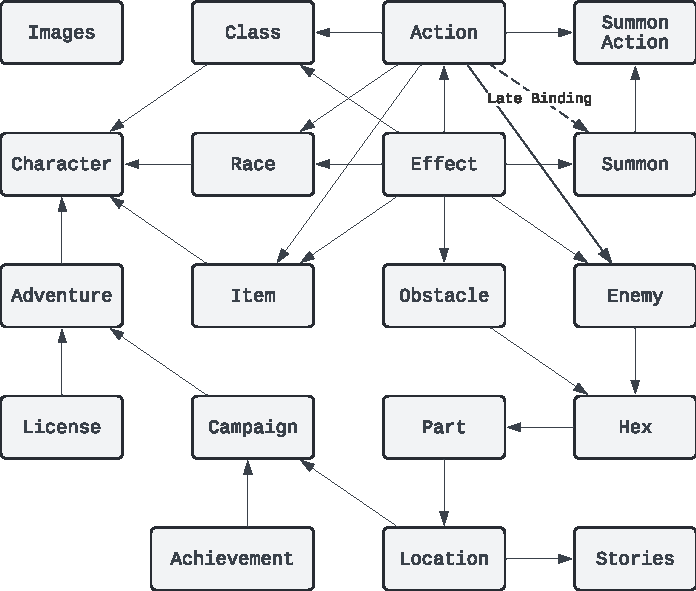
\includegraphics[width=0.7\textwidth]{diagrams/databasePriority}
    \caption{Schéma závislosti tabulek v databázi}
    \label{fig:db_table_priority}
\end{figure}

\begin{table}[H]
    \centering
        \begin{tabular}{l c l}
            \toprule

            \textbf{Název tabulky} & \textbf{Priorita} & \textbf{Závislost} \\
            \midrule

            \textbf{Effect} & 1 & -- \\
            \textbf{Achievement} & 1 & -- \\
            \textbf{Images} & 1 & -- \\
            \textbf{Parts} & 1 & -- \\
            \textbf{Obstacles} & 2 & Effect \\
            \textbf{Summons} & 2 & Effect \\
            \textbf{Enemies} & 3 & Effect, Action \\
            \textbf{Locations} & 3 & Part \\
            \textbf{Races} & 3 & Effect, Action \\
            \textbf{Items} & 3 & Effect, Action \\
            \textbf{Summons (Late Binding)} & 3 & Action \\
            \textbf{Campaigns} & 4 & Location, Achievement \\
            \textbf{Stories} & 4 & Location \\
            \textbf{Adventure} & 5 & License, Campaign \\
            \textbf{Characters} & 6 & Class, Race, Item, Adventure \\

            \bottomrule
        \end{tabular}
    \caption{Tabulka s prioritou dle Diagramu~\ref{fig:db_table_priority}
    \label{tab:db_table_priority}}
\end{table}

\section{Týmová spolupráce}
\label{sec:implementation-collaboration}
Týmová spolupráce ve čtyřčlenném týmu studentů se stává obzvláště komplikovaná v době, kdy je projekt rozdělen do separátních části, které jsou na sobě závislé a je nutná vzájemná komunikace a spolupráce. Jako hlavní a nejvíce důležitou komponentou tohoto projektu se stává API, která slouží pro kompletní komunikaci v rámci projektu. V této sekci se zaměřím na to, jak jsme si rozdělili práci a jaký software jsme k tomu využili.

\subsection{Rozdělení práce}
\label{subsec:implementation-collaboration-distribution}
Rozdělení práce v týmu bylo provedeno tak, že každý člen měl dle zadání přidělenou určitou hlavní část projektu, za kterou byl plně zodpovědný. Každá z těchto částí pak byla následně rozdělena na menší sekce, na kterých se daní členové podíleli buď samostatně, nebo ve spolupráci. Ta je zobrazena v šedém boxu, kde její vnitřní barevné čtverce reprezentují dané členy. Ve výsledném rozdělení práce na Obrázku~\ref{fig:job_distribution} je tak navíc jasně velikostně zobrazena náročnost jednotlivých částí projektu.

\begin{figure}[H]
    \centering
    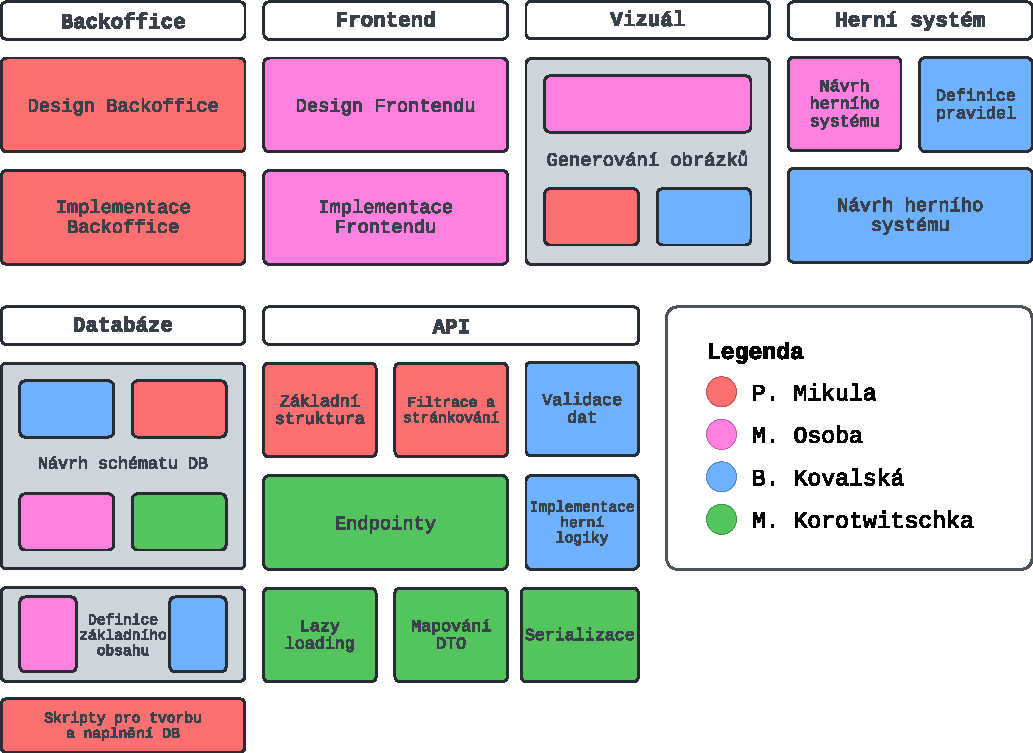
\includegraphics[width=0.95\textwidth]{../../shared/diagrams/blocks}
    \caption{Rozložení práce v týmu}
    \label{fig:job_distribution}
\end{figure}

\subsection{Verzování kódu}
\label{subsec:implementation-collaboration-versioning}
Efektivnost verzování kódu je důležitou součástí každé týmové spolupráce na větším projektu. Pro správu obsahu práce jsme využili nástroj Git pod službou GitHub\footnote{https://github.com/}, který nám umožnil efektivně sledovat změny a udržovat si přehled o vývoji projektu. Využití Gitu bylo zvoleno především pro jeho jednoduchost a znalost všech členů týmu, kteří s ním již měli zkušenosti v minulosti.

\subsubsection*{Větve}
\label{subsubsec:implementation-collaboration-versioning-branches}
V moderních vývojích systému se každá část nebo projekt rozděluje do složitějšího stromu větví. Tento proces je známý pod názvem \textit{Git Worfkflow}, jeho efektivní reprezentaci lze vidět na Obrázku~\ref{fig:git_workflow}. Tento strom se dělí na vícero větví, kde mezi ty hlavní tři patří \textit{live} neboli master, \textit{develop} a \textit{uat} (User Acceptance Testing) známá jako testing branch.

Větev \textit{master} slouží pro produkční verze projektu, které jsou již plně připraveny k nasazení, zatímco větev \textit{develop} slouží pro vývoj nových funkcí případně oprav chyb. Při vývoji nové funkce se pak každá tato aktualizace dostává pomocí tzv. \textit{pull requestu} do větve testovací. V této větvi pak dochází ke konstantnímu testování celého systému a pokud je vše v pořádku, aktualizace se dostávají do produkční větve.

Následně strom obsahuje pod větve vývojové, které se štěpí z větve developu a slouží pro vývoj nových funkcí nebo opravu chyb. Po dokončení a úspěšném testování je tato větev spojena zpět do developu a po vydání nové verze je spojena do masteru.

\subsubsection*{Zkratky}
Tabulka zkratek je zobrazena v Obrázku~\ref{fig:git_workflow}. Nejedná se zde o funkční příkazy softwaru Git, ale o pouhé zkratky pro přehlednější vyobrazení v schématu.

\begin{table}[H]
    \centering
    \resizebox{\textwidth}{!}{%
        \begin{tabular}{l l l}
            \toprule

            \textbf{Příkaz} & \textbf{Zkratka} & \textbf{Význam} \\
            \midrule

            \textbf{git nh} & New Hotfix & Vytvoření větve pro rychlou opravu chyb, která je již v produkci \\
            \textbf{git mh} & Merge Hotfix & Dokončení opravy chyby a spojení větve zpět do masteru \\
            \textbf{git live} & Release & Publikace nové verze a spojení větve do masteru \\
            \textbf{git nb} & New Bugfix & Vytvoření větve pro opravu chyb, která je ve vývoji \\
            \textbf{git mb} & Merge Bugfix & Dokončení vývoje a spojení větve zpět do developu \\
            \textbf{git uat} & User Acceptance Testing & Vytvoření větve pro testování nové verze \\
            \textbf{git nf} & New Feature & Vytvoření větve pro vývoj nové funkce \\
            \textbf{git mf} & Merge Feature & Dokončení vývoje a spojení větve zpět do developu \\

            \bottomrule
        \end{tabular}}
    \caption{Seznam zkratek pro větve v Git Workflow dle Obrázku~\ref{fig:git_workflow}
    \label{tab:git_workflow}}
\end{table}

\begin{figure}[H]
    \centering
    \includegraphics[width=0.9\textwidth]{figures/GitWorkflow}
    \caption{Ukázka správného použití verzovacího systému Git \cite{git_workflow}}
    \label{fig:git_workflow}
\end{figure}

\subsection{Sdílení kódu}
\label{subsec:implementation-collaboration-sharing}
Sdílení kódu není ve vývoji softwaru novinkou, neboť kód ve větším týmu spravuje vícero programátorů. Pro náš účel jsme opět použili systém \textit{GitHub}\footnote{https://github.com/}, kde po založení organizace dostávají všichni členové možnost zapojit se do vývoje. Obrázek~\ref{fig:git_organization} zobrazuje reprezentaci organizace na webové stránce \textit{GitHub}\footnote{https://github.com/Trails-Through-Shadows}, v níž jsou zobrazeny jednotlivé části projektu, jejich krátký popis a jazyk, který v dané části převládá.

\subsection*{Rozdělení částí}
\label{subsec:implementation-collaboration-sharing-parts}
Při zakládání organizace také došlo k zakoupení domény, na kterou následně byly jednotlivé produkční verze nasazeny pomocí dalšího z nástrojů GitHubu a to \textit{GitHub Actions}\footnote{\href{https://github.com/features/actions}{https://github.com/features/actions}}, který slouží pro automatizaci testování a následného nasazení funkční verze na server. Tento systém nám umožnil přehledný a automatický proces spuštění aplikace v praxi.

\noindent
V rámci organizace byly vytvořeny následující části:

\begin{itemize}
    \item TTS-Thesis    -- obsahuje texty diplomové práce od jednotlivých členů týmu se sdílenými materiály, který se nachází pod odkazem \url{https://docs.tts-game.fun/thesis/intro}.
    \item TTS-Database  -- obsahuje skripty pro vytvoření a naplnění databáze základními daty, jejichž schéma je viditelné na Obrázku~\ref{fig:db_scheme} nebo pod odkazem \url{https://db.tts-game.fun}.
    \item TTS-API       -- obsahuje zdrojové kódy API, které slouží pro komunikaci mezi frontendem a backendem. Funkční produkční verze běží pod odkazem \url{https://api.tts-game.fun}.
    \item TTS-Dashboard -- obsahuje zdrojové kódy frontendu, který slouží pro zobrazení dat a správu aplikace. Produkční verze nalezena pod odkazem \url{https://dashboard.tts-game.fun}.
    \item TTS-Frontend  -- obsahuje frontend, který slouží pro interakci s uživatelem. Produkční verze dostupná na \url{https://play.tts-game.fun}.
    \item TTS-Docs      -- obsahuje dokumentaci k projektu která je volně dostupná pod odkazem \url{https://docs.tts-game.fun/data/intro}.
\end{itemize}

\begin{figure}[H]
    \centering
    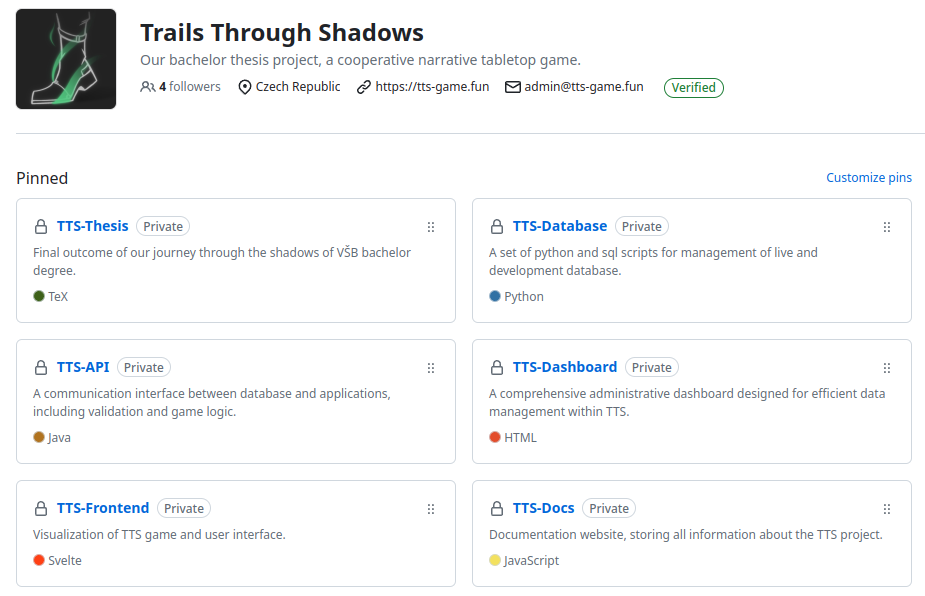
\includegraphics[width=0.9\textwidth]{../../shared/figures/gitOrg}
    \caption{Zobrazení organizace a jejich částí na stránce Github}
    \label{fig:git_organization}
\end{figure}

\subsection{Řešení problémů}
\label{subsec:implementation-collaboration-problems}
Pro řešení problému a chyb v softwaru bylo pro tuto práci využito dalšího z nástrojů webu Github a to konkrétně \textit{Github Issues}\footnote{\href{https://github.com/features/issues}{https://github.com/features/issues}}, který slouží pro ukládání a monitoring problému v projektu. Jako jednu z výhod tento nástroj přináší možnost přiřazení problému danému členovi nebo automatické vytvoření \textit{feature} větve a následného \textit{pull requestu}.

\section{Problémy vývoje}
\label{sec:implementation-problems}
Během vývoje aplikace se vyskytlo mnoho menších a větších problémů, které bylo nutné řešit a následně eliminovat. V této sekci práce se tak zaměřím na ty větší problémy, které přinesly největší výzvu během vývoje.

\subsection*{Hexagonální grid}
\label{subsec:implementation-problems-hexagon}
Během implementace bylo nutné vykreslit hexagonální mapu, která slouží jako základ pro reprezentaci lokace, například jeskyně (z anglického \textit{dungeon}). Tato mapa reprezentuje bojové pole, kde se odehrává herní děj, a je tedy nezbytné správně zaznamenat polohu každého objektu na mapě do databáze, včetně umístění každého hexagonu na plánku, který byl zobrazen.

Při používání hexagonálního rozložení bylo nezbytné načítat z databáze veškeré hexagony, jejich sousedy a vazby, které obsahují s dalšími objekty. Po několika pokusech s klasickými souřadnicemi ve formátu \textit{(x, y)} nám bylo doporučeno přejít na souřadnicový systém osový, známý jako \textit{axial coordinates}, který je reprezentován formátem \textit{(q, r, s)}. Tento systém je používán právě v hexagonálních hrách, protože usnadňuje výpočet vzdálenosti mezi hexagony a identifikaci jejich sousedů pomocí třetí osy.

Pro ověření správnosti souřadnic je možné sečíst všechny souřadnice hexagonu, které by měly dát výsledek 0. Tento výpočet je zobrazen v Rovnici~\ref{eq:axial-coordinates-verification}.
\begin{equation}
    q + r + s = 0\label{eq:axial-coordinates-verification}
\end{equation}

Hexagon jako samotný má možnost mít šest sousedů, které lze vidět na obrázku vedle Rovnice~\ref{eq:hexagon-neighbors}. V případě použití normálního souřadnicového systému by bylo zapotřebí vytvořit složitý algoritmus pro výpočet sousedů, zatímco v případě osových souřadnic stačí ke každému koordinátu přičíst nebo odečíst číslo 1. Výpočet sousedů je zobrazen v Rovnici~\ref{eq:hexagon-neighbors}. \cite{hexagon_grid}

\begin{equation}
    \vcenter{\hbox{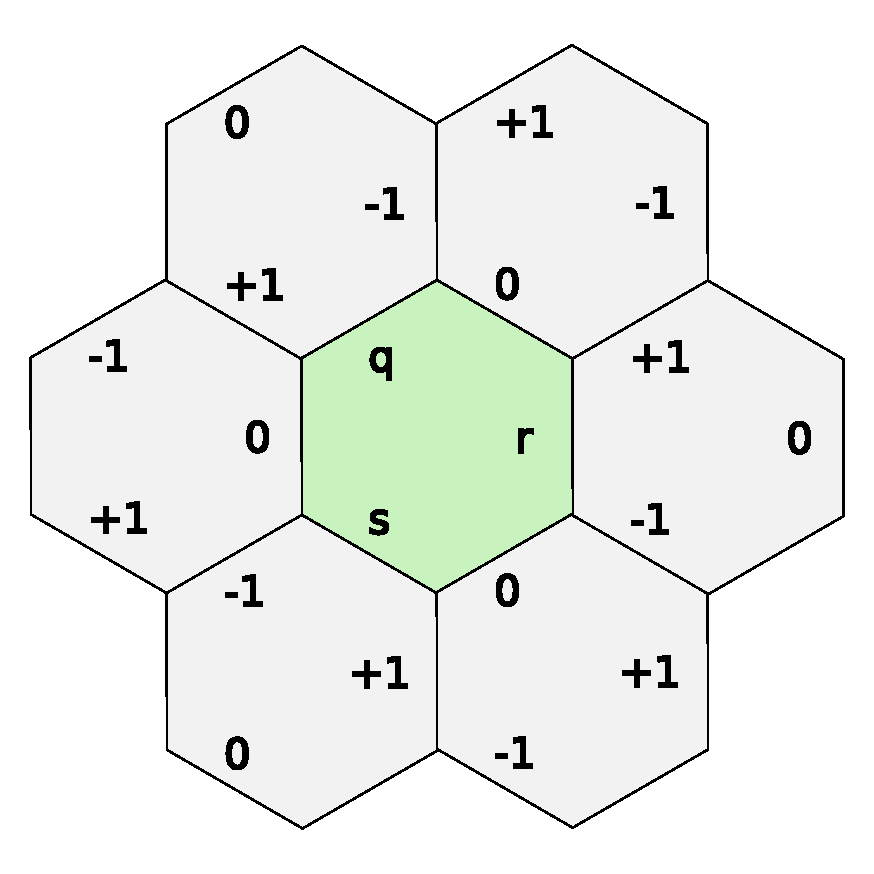
\includegraphics[width=6cm,height=6cm]{diagrams/hexagonNeighbors}}}
    \qquad\qquad
    \begin{aligned}
        \text{Vrchní Levý} & : (q, r - 1, s + 1) \\
        \text{Vrchní Pravý} & : (q + 1, r - 1, s) \\
        \text{Levý} & : (q - 1, r, s + 1) \\
        \text{Pravý} & : (q + 1, r, s - 1) \\
        \text{Dolní Levý} & : (q - 1, r + 1, s) \\
        \text{Dolní Pravý} & : (q, r + 1, s - 1)
    \end{aligned}\label{eq:hexagon-neighbors}
\end{equation}

\subsection*{Časová náročnost}
\label{subsec:implementation-problems-time}
Dalším z problémů, který byl zaviněn špatným návrhem byla časová náročnost aplikace. Vzhledem k tomu, že návrh projektu byl proveden bez zohlednění časové náročnosti, pro dokončení práce bylo zapotřebí vynechat několik funkcí, mezi které patří implementace \textit{summons}, \textit{items}, \textit{achievements} a také správa uživatelských dat, které byly původně plánovány jako součást hry.

K této funkcionalitě bychom se v budoucnu rádi vrátili a implementaci dokončili.

\subsection*{Chyba volby frameworku}
\label{subsec:implementation-problems-framework}
Během vývoje rozhraní se postupně nabalovaly problémy, které vybraný framework obsahoval. Jeho volba totiž nebyla dostatečně promyšlená a nebyl zohledněn fakt, že i administrativní rozhraní obsahuje část uživatelskou. Z tohoto důvodu by bylo vhodné zvolit jiný framework, který se více zaobírá frontendem.

V raných fázích vývoje byl zvolen framework Django, který byl ze všech možností nejvíce známý, neboť jsem s ním pracoval v rámci studia. Později v konečném semestru studia jsem vykonal předmět zaměřující se mimo jiné na framework React, který se okamžitě projevil jako lepší varianta pro psaní administrativního rozhraní. Bohužel vzhledem k časové náročnosti a nedostatku zkušeností s frameworkem React, bylo rozhodnuto zůstat u frameworku Django. Jedná se tedy o chybu, která by mohla v případě pokračování vývoje způsobit problémy.

\endinput

% Zaver
\chapter{Závěr}
\label{ch:conclusion}

V této bakalářské práci jsme se zaměřili na návrh a implementaci administrativního rozhraní pro kompletní správu obsahu výpravně evoluční hry, která tak kombinuje prvky deskových a digitálních her. Cílem práce bylo vytvořit efektivní nástroj umožňující administrátorům správu herních prvků, jako jsou postavy, předměty, lokace, nepřátele a další. V průběhu práce byla provedena analýza existujících administrativních rozhraní zaměřená na jejich funkčnost a uživatelskou přívětivost, na základě které byla výsledná práce směřována.

Implementace administrativního rozhraní tak zahrnovala vytvoření funkčního prototypu, který umožňuje provádět operace nad objekty, jako je vytváření, editace, mazání nebo zobrazení detailů. Prototyp tak byl vyvíjen s obezřetnosti na možnost budoucího rozšíření a modulárnosti. Díky kombinaci moderních technologií bylo možné vytvořit uživatelsky přívětivé rozhraní s intuitivní navigací a bezpečnostními opatřeními.

Součástí této práce se tak dá považovat i spolupráce s ostatními členy týmu na vývoji herního designu, implementaci API nebo tvoření celkového obsahu hry, který lze vidět v zdrojových kódech přílohy \textit{TTS-Database}.

Kromě technické implementace byla také vytvořena uživatelská příručka, které je samostatně integrovaná do administrativního rozhraní. Uživatelskou příručku tak lze naleznout v kterékoliv sekci webu pod tlačítkem \textit{Help}. Tento manuál tak poskytuje dostatečné informace, které uživatelům umožňují efektivně využívat všechny funkce rozhraní.

Celkově tak lze konstatovat, že výsledný prototyp splňuje veškeré stanovené cíle dle zadání a představuje tak schopný nástroj pro správu obsahu hry. Díky možnostem rozšíření tak není v budoucnu problém rozhraní rozšířit o další aktualizace. Budoucí práce by tak mohla zahrnovat rozšíření o další nástroje jako je například statistika, záznam provedených akcí nebo celkově rozšířit možnost efektivněji spravovat obsah.

Ukázka výsledného rozhraní je možné vidět v příloze~\ref{ch:appendix-interface-screenshots}

\endinput

% Prilohy
\appendix

% Seznam literatury
\printbibliography[title={Literatura}, heading=bibintoc]

\end{document}
